\begin{titlepage}
    \centering
    \vspace*{\fill}

    \vspace*{0.5cm}

    \Large% \bfseries
    Análise de longo prazo (1985 – 2018) das mudanças florestais na Mata Atlântica utilizando o algoritmo Landtrendr

    \vspace*{5cm}

    % \large Eduardo Ribeiro Lacerda

    \vspace*{\fill}
\end{titlepage}

\section{Análise de longo prazo (1985 – 2018) das mudanças florestais na Mata Atlântica utilizando o algoritmo Landtrendr}

% \begin{abstract}
%     abstract
% \end{abstract}

\subsection{Introdução}
\hspace{13pt} Estamos na década da restauração (2020 - 2030), e o desafio para alcançar as metas são enormes. A Mata Atlântica, como uma das regiões mais biodiversas do mundo \citep{REZENDE2018208}, tem papel importante nesse desafio. Movimentos como a criação do Pacto pela Mata Atlântica em 2009 visando a restauração de 15 Mha de áreas degradadas até 2050, servem para mostrar a importância que o bioma tem para a conservação da parte considerável da biodiversidade mundial com suas quase 16 mil espécies de plantas e mais de 2 mil espécies de vertebrados \citep{scarano2014}.  

O bioma está entre as áreas com maior biodiversidade do mundo ao mesmo tempo que também é considerada uma das mais ameaçadas e historicamente degradadas. A restauração dessas áreas está diretamente associada a forma com que os atores associados irão lidar com dificuldades como o custo de implementação da restauração, interesses econômicos locais, falta de investimento, assistência técnica limitada e baixo nível de governança em algumas regiões \citep{strassburg_strategic_2019, CROUZEILLES2019, Chazdon2017, Strassburg2020}. 

Como os compromissos nacionais e internacionais possuem metas para conservação e restauração, o entendimento sobre a dinâmica do uso e cobertura do solo nessas regiões passou a ser ainda mais importante. O desenvolvimento de técnicas que ajudam a entender os processo através da incorporação do tempo nas análises são essenciais para o acompanhamento dos projetos, assim como para o próprio estabelecimento das metas. Entender o quanto se deve restaurar tem ligação direta com o que foi perdido em ações antrópicas recentes. Quantificar as mudanças para estabelecer metas e qualificar as perdas para justificar os compromissos. Entender os processos para compreender os fluxos e o sentido das dinâmicas no espaço. Estas são tendências na área de geotecnologia e a consequência vem sendo o desenvolvimento de ferramentas e soluções geoespaciais que visam possibilitar a análise e até mesmo o monitoramento do espaço no tempo.

A Mata Atlântica, assim como a Amazônia, é um dos biomas mais estudados no território nacional. Devido ao contexto histórico do processo de colonização brasileiro, o bioma foi o primeiro a ser ocupado e hoje possui 70\% da população do pais, além de possuir apenas cerca de 27\% de sua área preservada \citep{Carla2008}, quase sempre de forma bastante fragmentada. Mapeamentos de alta precisão \citep{Carla2008}, assim como projetos de mapeamento sistemático \citep{Souza2019}, vem sendo condizidos no bioma, mas a qualificação dos eventos tradicionalmente só é feita após os resultados serem obtidos. Consequentemente, esta qualificação do resultado acaba sendo feita de forma limitada de acordo com o dado gerado. Se o dado final apresenta apenas os eventos de mudança e a data da detecção, não há muito mais o que extrair do que apenas a quantificação das áreas, a data da mudança e o sentido restrito das tendências de mudança.

A identificação das mudanças através da comparação binária entre datas não consegue compreender a complexidade de processos principalmente em regiões mais dinâmicas como a Mata Atlântica. Para além da identificação da mudança em si, é cada vez mais necessário identificar a magnitude dos eventos, sua duração, sua amplitude e até mesmo a quantificação de diversos eventos de mudança em uma mesma região como viabilizador para análises de resiliência \citep{Jakovac2015}. Visando possibilitar estas análises, ferramentas especializadas vem sendo desenvolvidos na última década. Exemplos como o CCDC \citep{ZHU2014152}, COLD \citep{Cohen2020}, VCT \citep{Huang2010, THOMAS201119} , VerDET \citep{Hughes2017}, EWMACD \citep{Brooks2014}, MIICA \citep{JIN2013159}, ITRA \citep{VOGELMANN201292}, Shapes-NBR \citep{Meyer2013, Moisen2016} e o Landtrendr \citep{KENNEDY20102897, KENNEDY2012117} podem ser citados.
Dentre eles, o possivelmente mais popular, principalmente desde sua implementação na plataforma Google Earth Engine (GEE) \citep{Kennedy2018}, é o Landtrendr.

No entanto, apesar de sua implementação inicial ter surgido a mais de uma década \citep{KENNEDY20102897}, a análise de áreas de grande extensão com a da Mata Atlântica, eram inviáveis, vide a capacidade computacional necessária tanto para o processamento dos dados de entrada quanto para a execução do próprio algoritmo. O surgimento de uma plataforma como o Google Earth Engine \citep{GORELICK201718} possibilitou a escalabilidade necessária. Algoritmos como o Landtrendr deixaram de lado a comparação direta entre classes e focaram na execução de modelos de regressão possibilitando uma análise temporal, como uma busca para uma melhor qualificação dos resultados, para que cada pixel possa contar uma história um pouco mais completa desse espaço.

Devido a possibilidade de uso de ferramentas como as citadas, e visando uma melhor qualificação dos eventos de mudança em áreas que tiveram ou ainda possuem área de floresta, o presente trabalho teve como objetivo o uso do algoritmo Landtrendr na plataforma GEE para o mapeamento de todos os eventos de perda e de ganho de floresta em toda a região da Mata Atlântica em território nacional. Para além do próprio mapeamento, o trabalho teve como objetivo a quantificação e qualificação das dinâmicas ocorridas na região de 1985 até 2018 buscando entender as dinâmicas espaciais no âmbito do bioma e também de acordo com as divisões políticas. As divisões espaciais da análise visam contribuir não só com o conhecimento sobre os eventos ocorridos nos últimos 33 anos em todo bioma quanto para tomadas de decisão políticas em âmbito estadual e até mesmo municipal. 

\subsection{Materiais e Métodos}
\subsubsection{Dados de entrada}
\hspace{13pt} Para este estudo foram utilizadas imagens do satélite Landsat da série 5, 7 e 8 com valores de reflectância da superfície de 1985 até 2018. Para cobrir toda a área do bioma da Mata Atlântica foram necessárias 88 cenas (path/row) diferentes, cada cena contendo 23 imagens por ano, por 33 anos, o que resultou em um total de aproximadamente 67 mil imagens. Todas as imagens utilizaram o algoritmo Fmask para retirar sombras e locais com presença de nuvem antes da construção das composições anuais. 

O Landtrendr trabalha analisando uma banda ou índice por vez, sendo assim, para este trabalho, o índice NDVI foi escolhido e consequentemente extraído das composições anuais. As 88 cenas, cada uma com 33 índices NDVI, representando cada um dos anos da análise, foram utilizados como dado de entrada para o algoritmo. 

\subsubsection{Processamento dos dados}
\hspace{13pt} Todo o processamento do Landtrendr foi feito na plataforma do Google Earth Engine e exportado para um ambiente \textit{offline} para a etapa de pós-processamento, análise e validação. Toda o pós-processamento e análise foi feito utilizando a linguagem de programação R e a etapa de validação no \textit{software} TimeSync \citep{COHEN20102911}.

O processamento foi dividido com o objetivo de gerar resultados tanto para perda quanto para o ganho de áreas de floresta no bioma. Foram analisadas apenas áreas com vegetação de floresta. Para as análise de perda foram analisadas áreas que possuíam floresta em 1985 de acordo com o projeto Mapbiomas \citep{Souza2019} v4 e que não apresentaram recuperação da vegetação de acordo tanto com o Mapbiomas como quanto pelo próprio resultado da análise de ganho do Landtrendr. Já para a análise de ganho, foram retiradas primeiramente todas as áreas de floresta consideradas pseudo-invariantes, ou seja, áreas que foram classificadas como floresta pelo projeto Mapbiomas em todos os anos de 1985 até 2018 com o objetivo de excluir detecção de mudanças relacionadas a regeneração natural de florestas mais antigas que o tempo de análise do trabalho. Para o ganho, também foram retirados todos os pixels detectados pelo Landtrendr que tinham uma duração menor do que 4 anos, com o objetivo de mostrar áreas que tiveram um tempo mínimo de recuperação para serem consideradas florestas secundárias iniciais de acordo com a bibliografia especializada \citep{Chazdon2014}.

\subsection{Resultados e Discussões}
\hspace{13pt} Os resultados obtidos mostram uma Mata Atlântica com concentrações de perda na parte sul e nordeste do pais, e com ganhos locais distribuídos por todo o bioma. A Mata Atlântica que foi desmatada e fragmentada ao longos dos séculos se vê hoje ganhando mais do que perdendo em área total, mas as perdas e os ganhos não podem ser tratados de forma igualitária. A perda interfere mais na manutenção do bioma por degradar majoritariamente áreas antigas e bem estruturadas, enquanto os ganhos, por serem eventos ainda recentes, são frágeis e não possuem a mesma resiliência. Os resultados obtidos corroboram com outros estudos recentes como em \citep{Rosa2021, CROUZEILLES2019, REZENDE2018208}.  

\subsubsection{Resultados para os eventos de perda na Mata Atlântica}
\hspace{13pt} Somando-se todos os eventos de perda detectados pelo algoritmo após as filtragens das áreas de interesse, houveram ao longo de todos os anos da análise 61.167.796 de pixels com uma perda média de magnitude de 225 ou diminuição de 0.225 no índice NDVI. Isso equivale a uma área total de pouco mais de 55 mil $ km^2 $ de florestas que sofreram perdas significativas no bioma e que não foram recuperadas após a supressão.

O resultado mais abrangente envolvendo todos os eventos de perda do bioma pode ser visualizado na (Figura \ref{fig:heat_loss_masked85_maskedgain}). A maior aglomeração de eventos de perda está localizada principalmente entre os estados do Paraná e Santa Catarina e no estado da Bahia. Nos outros estados o mapa de calor mostra uma distribuição mais homogênea dos eventos ao longo do território. 

\begin{figure}[H]
    \centering
    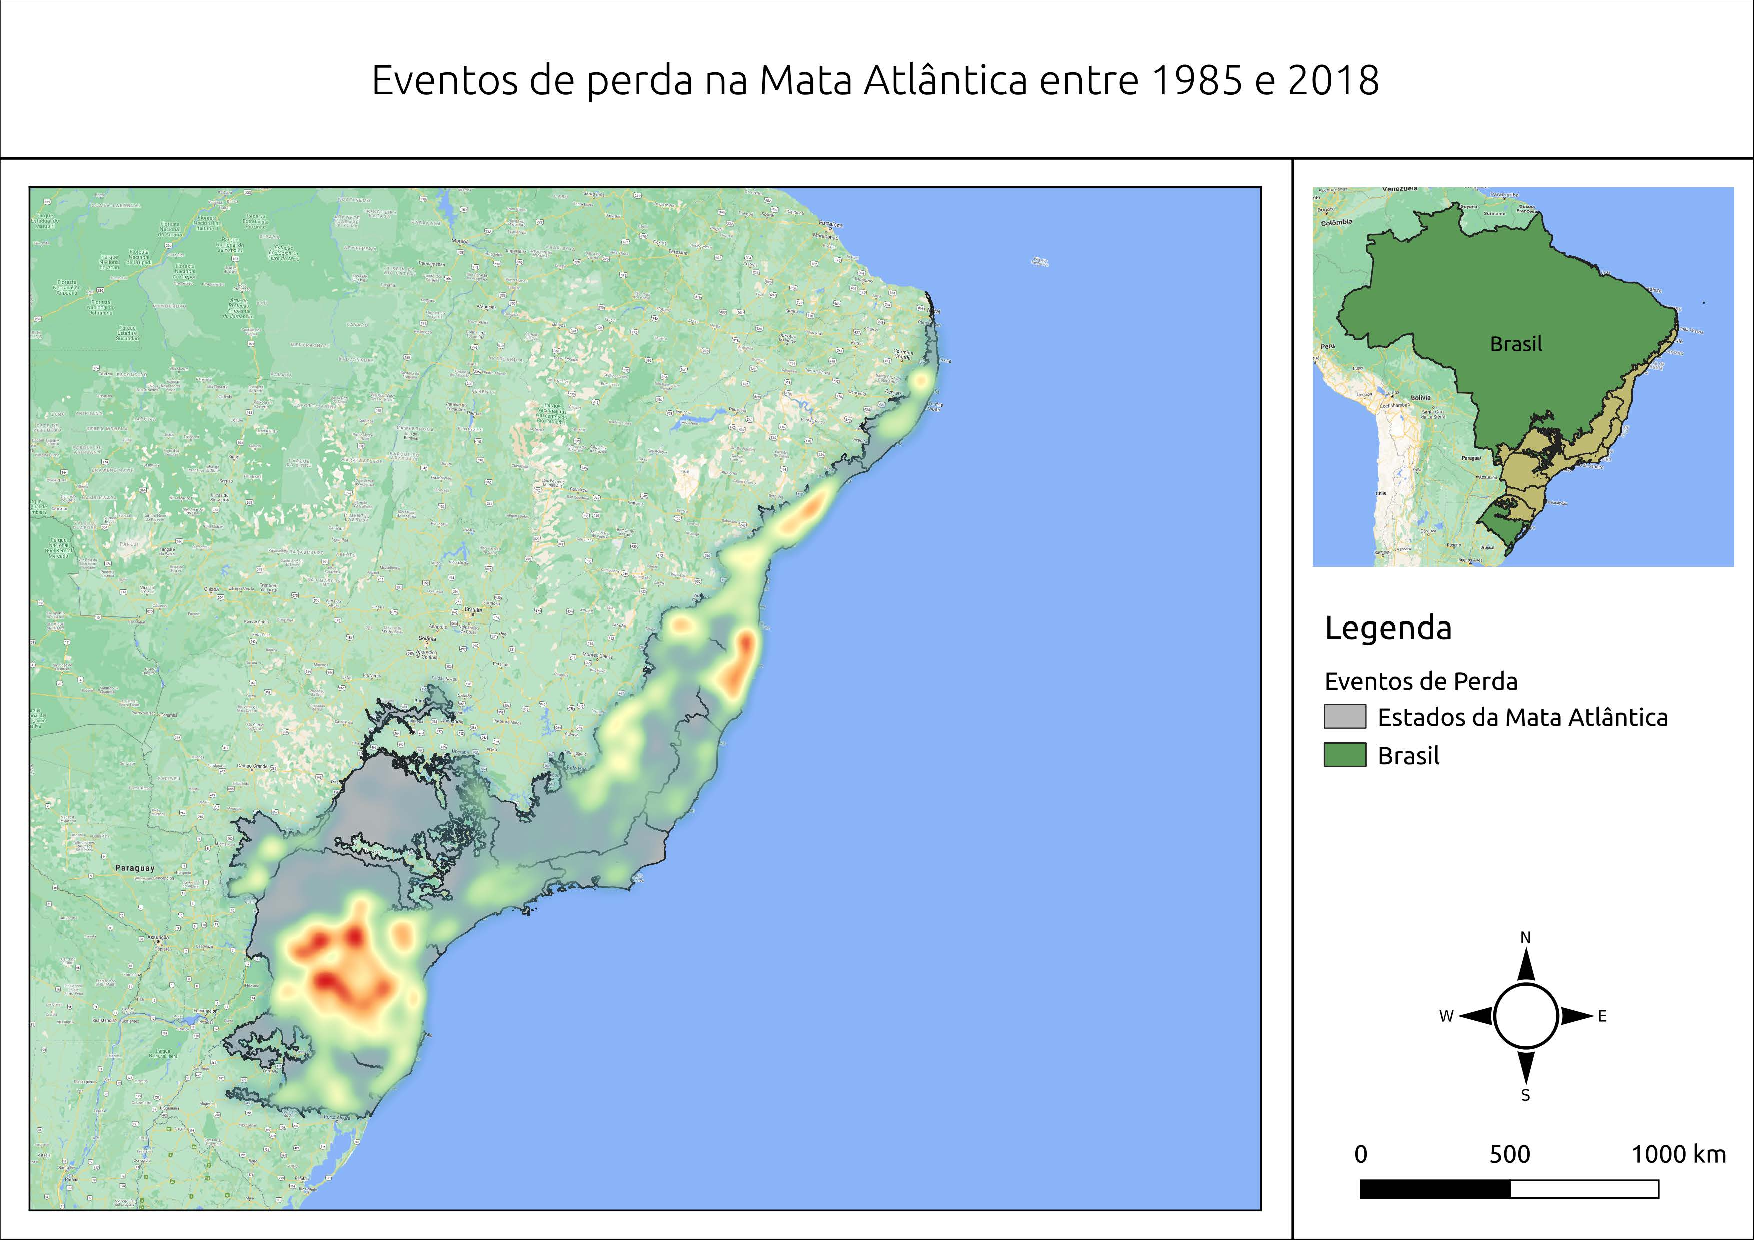
\includegraphics[scale=.5]{images/heatmap_loss_masked85_maskedgain.pdf}
    \caption{Todos os eventos de perda na Mata Atlântica entre 1985 e 2018.}
    \label{fig:heat_loss_masked85_maskedgain}
\end{figure}

Quando a divisão das detecções é feita de acordo com eventos de curta duração (um ano) e longos (maiores que um ano), verificamos que o padrão espacial das aglomerações (\textit{clusters}) se mantém semelhante com apenas algumas variações (Figura \ref{fig:heat_loss_eq1_neq1}). Os eventos de curta duração tendem a se localizar mais na fronteira entre Paraná e Santa Catarina, enquanto os de longa aconteceram com maior frequência na região central do Paraná, sul/norte da Bahia e norte de Pernambuco. Dos mais de 61 milhões de eventos detectados ou 55 mil $ km^2 $, cerca de 27.5 milhões foram eventos de curta duração, o que significa uma área aproximada de 25 mil $ km^2 $. Os outros 33.7 milhões de eventos tiveram duração maior que um ano, o que totalizou aproximadamente 30.4 mil $ km^2 $.

Já quando a divisão é feita por estados (Figura \ref{fig:estados_loss_masked85_maskedgain}), verificamos que estados como Minas Gerais possuem um número grande de eventos que estão distribuídos de forma homogênea pelo território, assim como Bahia e São Paulo. Vemos que apesar do maior \textit{cluster} de perdas estar localizado entre Paraná e Santa Catarina, a maior quantidade de eventos está no estado do Paraná. 

\begin{figure}[H]
    \centering
    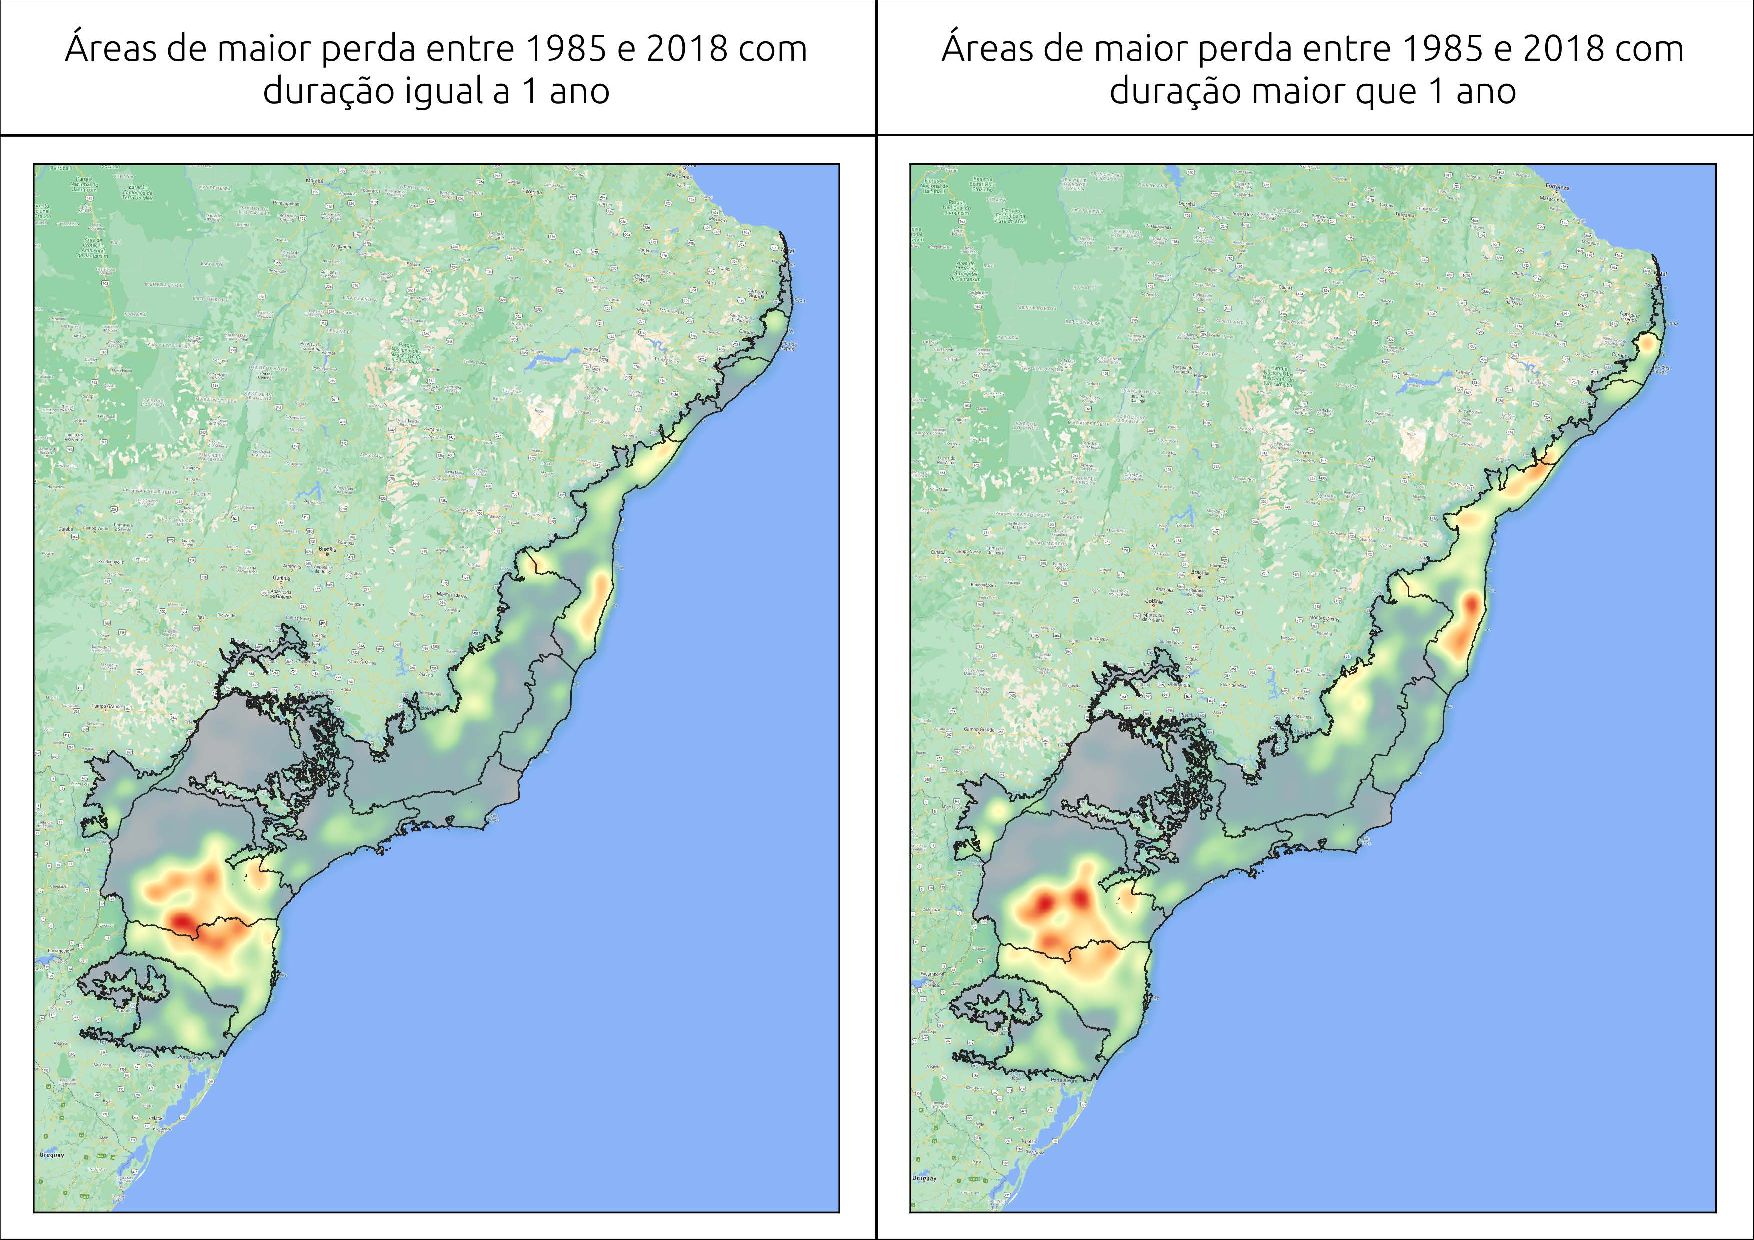
\includegraphics[scale=.5]{images/heatmap_loss_eq1_neq1.pdf}
    \caption{Mapa com os eventos de perda entre 1985 e 2018 tanto com duração igual a 1 quanto somente maiores que 1.}
    \label{fig:heat_loss_eq1_neq1}
\end{figure}

\begin{figure}[H]
    \centering
    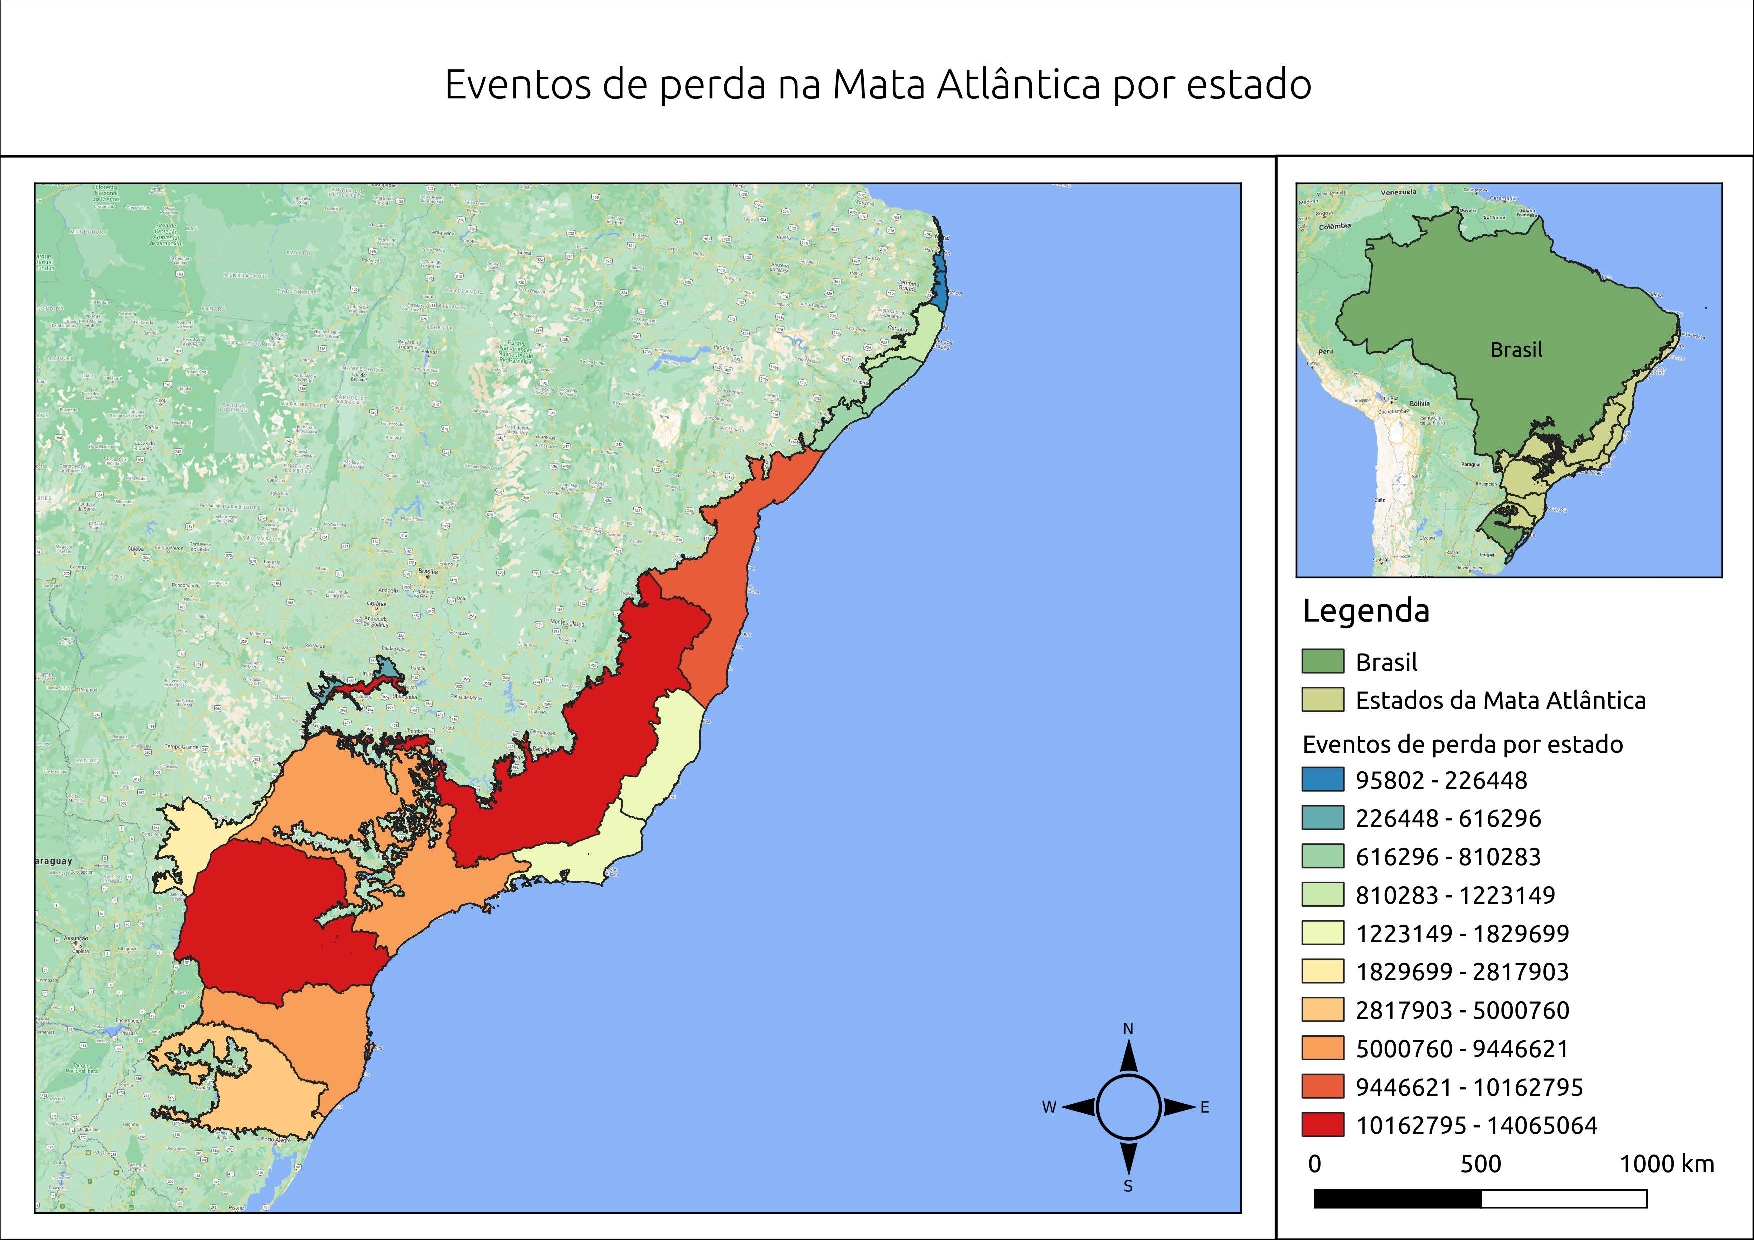
\includegraphics[scale=.5]{images/estados_loss_masked85_maskedGain.pdf}
    \caption{Todos os eventos de perda na Mata Atlântica entre 1985 e 2018 por estado. Os valores representam o número de pixels que tiveram alguma detecção de perda.}
    \label{fig:estados_loss_masked85_maskedgain}
\end{figure}

Ao considerar o número de eventos de acordo com a área de cada estado, verificamos que estados como Santa Catarina e Bahia se destacam mostrando o maior proporção de perdas ao longo dos 33 anos seguido de Pernambuco, Paraná e Sergipe (Figura \ref{fig:estados_loss_proporcional}). Já ao calcular a área perdida de acordo com a proporção de floresta presente em cada município em 1985, podemos perceber que grande parte do litoral nas regiões sul e sudeste mantiveram baixa proporção de perda com aumento significativo ao longo de parte majoritária do litoral nordestino (Figura \ref{fig:prop_loss}). \textit{Hotspots} com maior proporção podem ser identificados em todos os estados do nordeste, além de Paraná, Santa Catarina e Mato Grosso. Para este cálculo foram utilizados a quantidade total de pixels classificados como floresta pelo projeto Mapbiomas para o ano de 1985, assim como os pixels com os eventos de perda detectados durante todos os anos da análise. Uma proporção de 0,1 equivale a 10\% de perda da área total de florestas no município em 1985.

\begin{figure}[H]
    \centering
    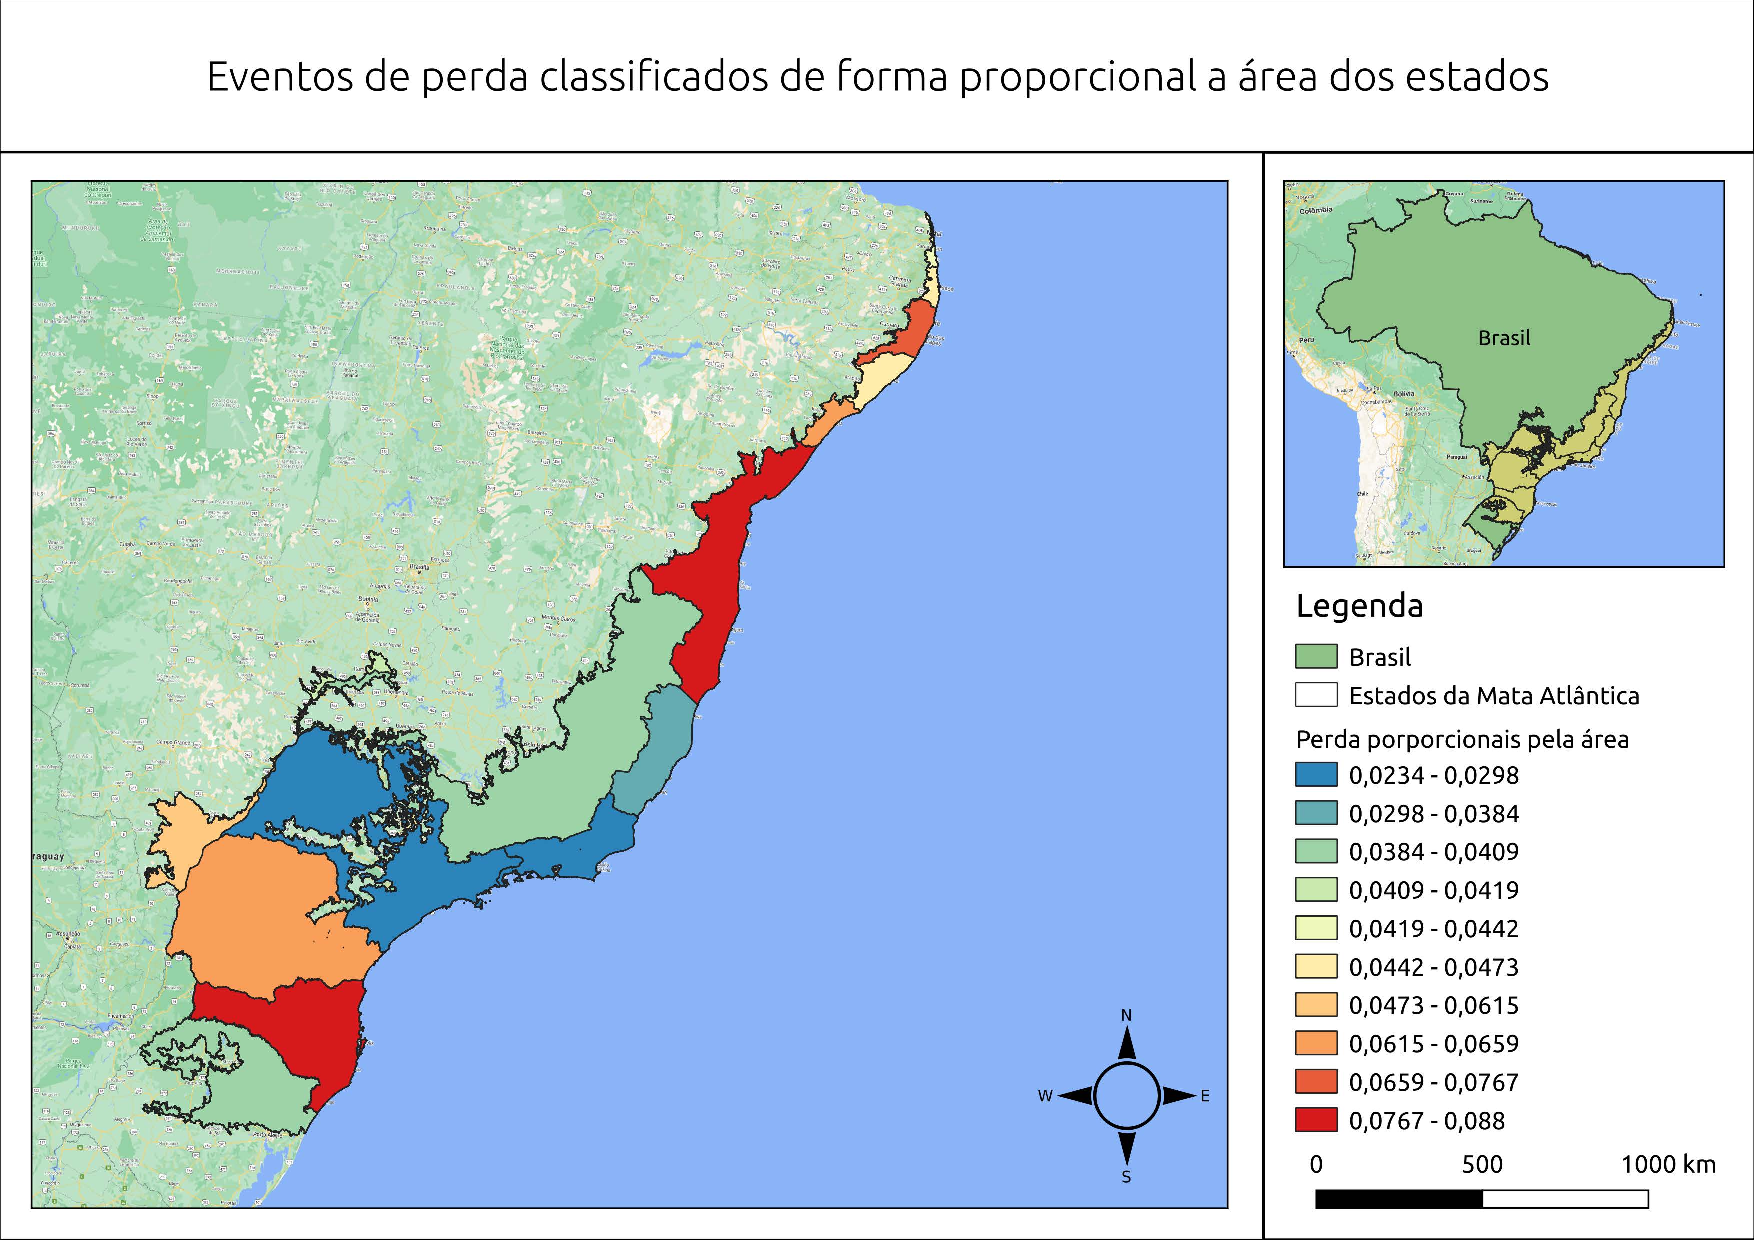
\includegraphics[scale=.5]{images/estado_loss_proporcional.pdf}
    \caption{Mapa com os eventos de perda entre 1985 e 2018 classificado de acordo com a proporção de área de cada estado.}
    \label{fig:estados_loss_proporcional}
\end{figure}

\begin{figure}[H]
    \centering
    \includegraphics[scale=.5]{images/prop_loss.pdf}
    \caption{Mapa com a proporção dos eventos de perda entre 1985 e 2018 classificado de acordo com a área total de floresta em 1985.}
    \label{fig:prop_loss}
\end{figure}

Já quando analisamos a proporção de área perdida dentro das unidades de conservação (UC) presente no bioma, percebemos que muitos eventos foram detectados durante a década de 1990. A tabela \ref{tab:uc_loss} mostra as dez unidades com maior quantidade de perda no bioma, a proporção de área de floresta perdida entre 1985 e 2018 em relação a área total da UC, o ano de criação da unidade e a média do YOD (\textit{Year of Detection}), ou seja, a média do ano de detecção dos eventos de maior perda detectado dentro das UCs. Esta coluna serve como parâmetro para entender se, em média, os eventos de mudança foram detectados antes ou depois da criação da UC. A UC com maior proporção de área perdida foi o Parque Nacional do Alto Cariri no estado da Bahia, que teve a maior parte dos seus eventos de perda detectados antes de sua criação em 2010.

\begin{table}[H]
    \centering
    \rowcolors{2}{red!50!yellow!30}{green!40!yellow!10}
    % \footnotesize
    \begin{tabular}{|c | c | c | c | c|}
    \hline
            Unidade de Conservação & UF & \% área perdida & Ano Criação & Média YOD \\
                PARNA do Alto Cariri & BA & 0.14 & 2010 & 1994 \\ 
                PARNA do Monte Pascoal & BA & 0.13 & 1961 & 1996 \\
                FLONA de Passo Fundo & RS & 0.13 & 1968 & 1992 \\
                ARIE Serra da Abelha & SC & 0.10 & 1990 & 1997 \\
                RESEX do Mandira & SP & 0.09 & 2002 & 1992 \\
                ESEC de Murici & AL & 0.09 & 2001 & 1991 \\
                FLONA de Canela & RS & 0.09 & 1968 & 1996 \\
                FLONA de São Francisco de Paula & RS & 0.08 & 1968 & 1994 \\
                FLONA de Assungui & PR & 0.07 & 1968 & 2004 \\
                FLONA de Caçador & SC & 0.07 & 1968 & 1995 \\
    \hline
    \end{tabular}
    \caption{As dez unidades de conservação com maior proporção de área perdida.}
    \label{tab:uc_loss}
\end{table}


Como visto previamente no mapa de \textit{clusters}, os eventos de perda de curta duração tendem a se concentrar principalmente no Paraná e Santa Catarina quando analisados sob divisões políticas (Figura \ref{fig:estados_loss_masked85_maskedgain_eq1}). Já os de longa duração, se concentram em estados como o Paraná e Bahia, seguido de Minas Gerais, Santa Catarina e São Paulo (Figura \ref{fig:estados_loss_masked85_maskedgain_neq1}).

Quando realizamos a divisão por municípios (Figura \ref{fig:mun_loss_masked85_maskedgain}), o padrão espacial similar ao mapa de calor da Figura \ref{fig:heat_loss_masked85_maskedgain}, mas demonstra como eventos que anteriormente estavam aparentemente distribuídos de forma mais homogênea, se agrupam quando classificados por município. As aglomerações ainda permanecem ocorrendo principalmente em estados como Paraná, Santa Catarina e Bahia, mas podemos observar municípios em outros estados que concentraram um maior número de perda como em Iguatemi no Mato Grosso do Sul ou em Águas Vermelhas em Minas Gerais. A lista completa com todos os 3078 municípios pertencentes ao bioma pode ser acessado neste link \url{https://github.com/sacridini/municipios_perdas_ganhos}.

\begin{table}[h!]
    \centering
    \rowcolors{2}{red!50!yellow!30}{green!40!yellow!10}
    % \footnotesize
    \begin{tabular}{|c | c | c|}
    \hline
                    Nome & Eventos & UF \\
            Porto Seguro & 444892 & BA \\
           Prudentópolis & 425340 & PR \\
              Ortigueira & 373635 & PR \\
 Coronel Domingos Soares & 367051 & PR \\
                Belmonte & 333728 & BA \\
               Itamaraju & 329167 & BA \\
              Guarapuava & 314087 & PR \\
     Santa Cruz Cabrália & 296493 & BA \\
                   Prado & 283573 & BA \\
             Canavieiras & 279240 & BA \\
    Rio Bonito do Iguaçu & 271232 & PR \\
                  Pinhão & 270471 & PR \\
            Encruzilhada & 264281 & BA \\
                 Reserva & 263798 & PR \\
                Bituruna & 262246 & PR \\
                  Tibagi & 253448 & PR \\
                   Mafra & 251392 & SC \\
           Santa Cecília & 246603 & SC \\
              Itaiópolis & 246205 & SC \\
              Guaratinga & 241392 & BA \\
    \hline
    \end{tabular}
    \caption{Os vinte municípios com maior número de eventos de perda}
    \label{tab:mun_loss}
\end{table}

\begin{figure}[H]
    \centering
    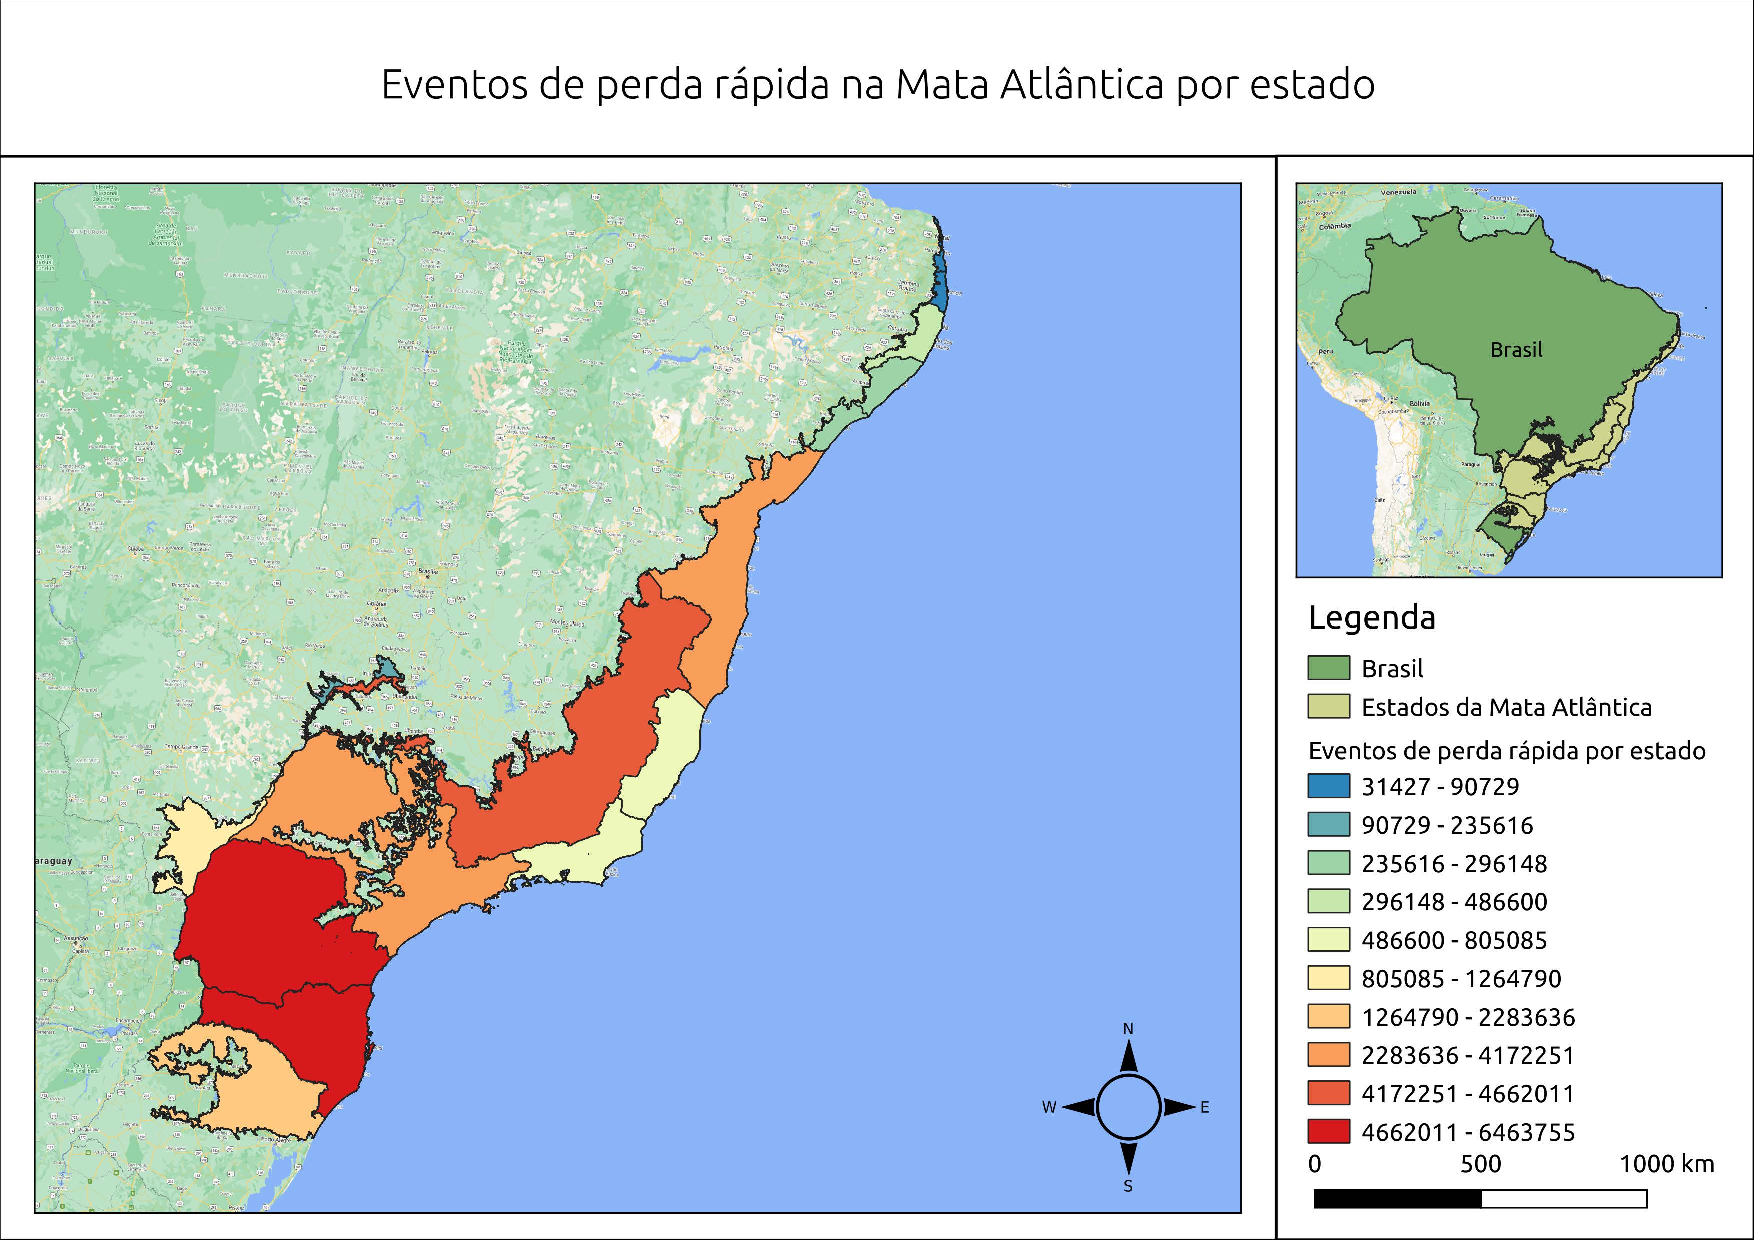
\includegraphics[scale=.5]{images/estados_loss_masked85_maskedGain_eq1.pdf}
    \caption{Todos os eventos de perda rápida (duração igual a 1) na Mata Atlântica entre 1985 e 2018 por estado. Os valores representam o número de pixels que tiveram alguma detecção de perda.}
    \label{fig:estados_loss_masked85_maskedgain_eq1}
\end{figure}

\begin{figure}[H]
    \centering
    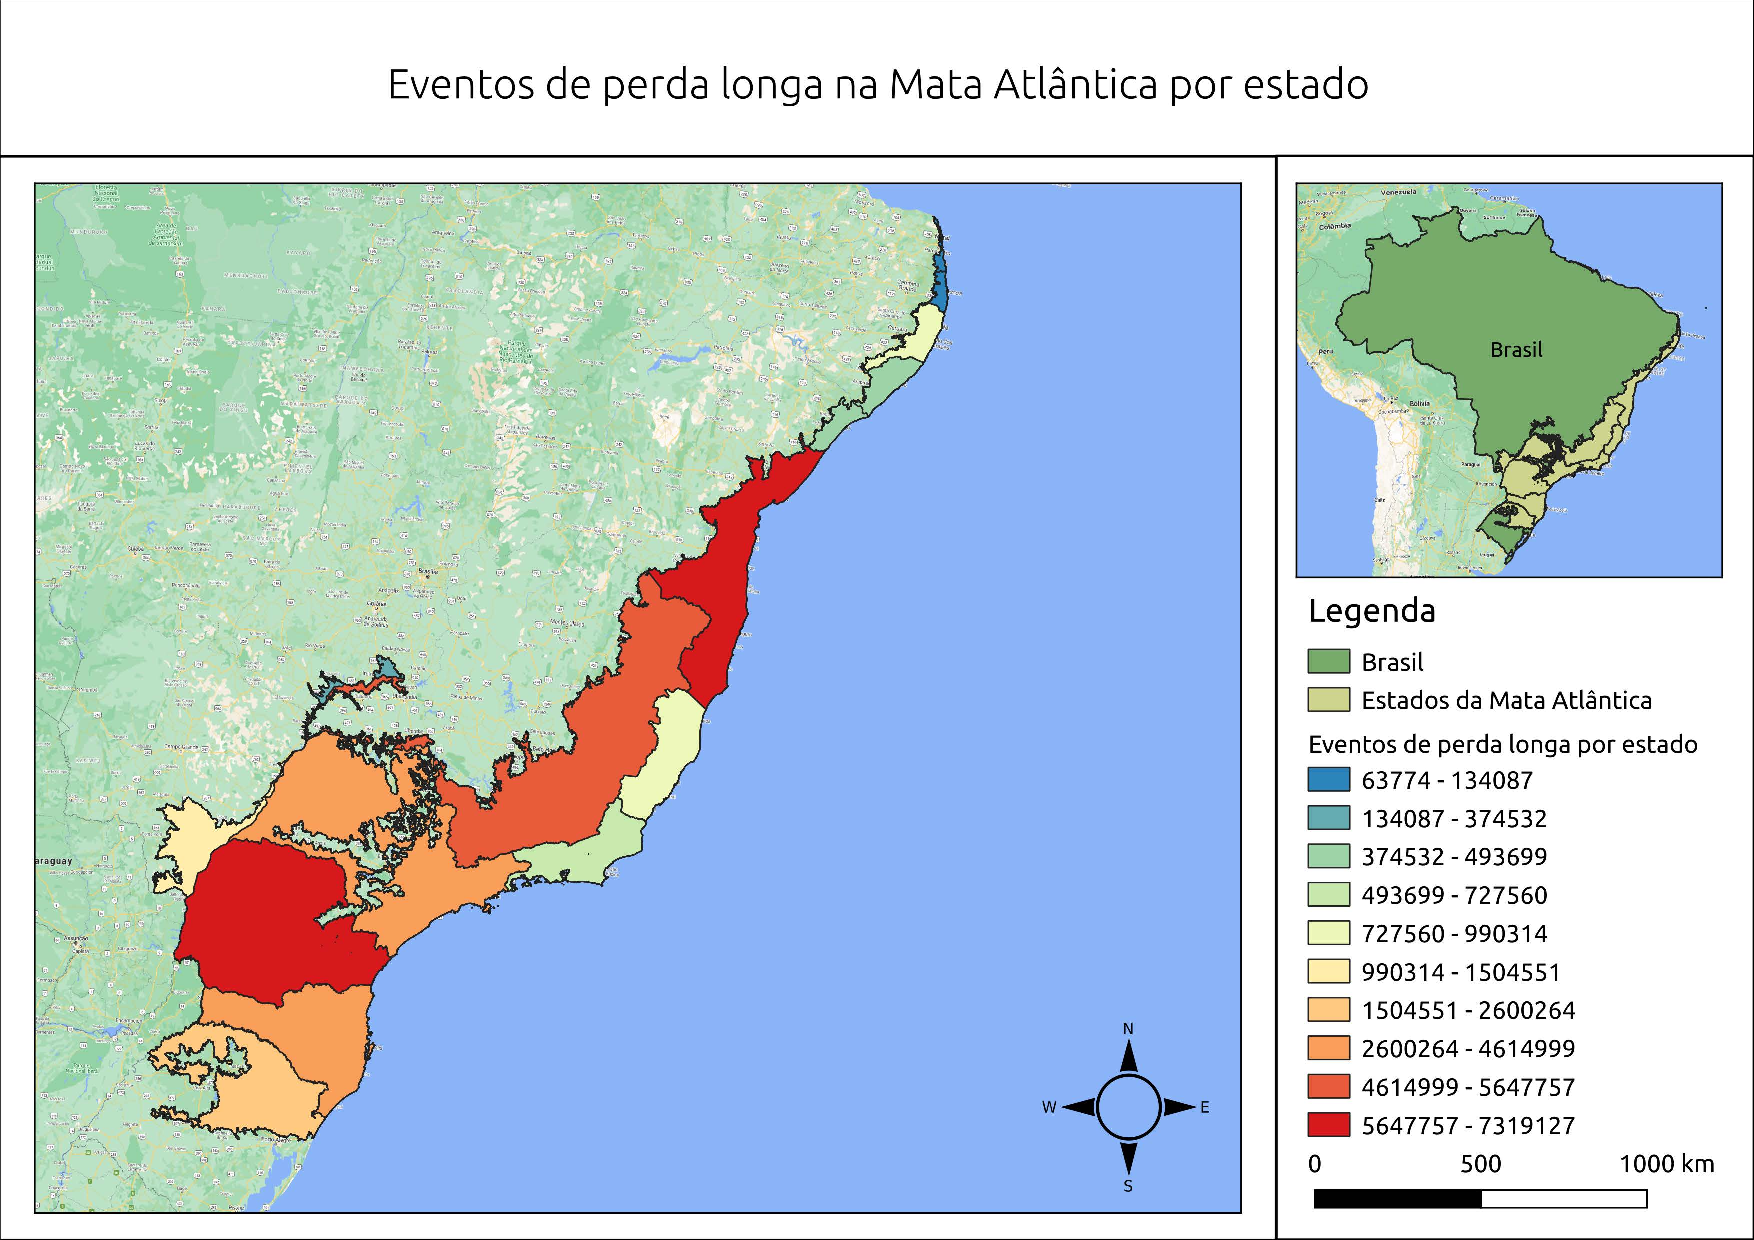
\includegraphics[scale=.5]{images/estados_loss_masked85_maskedGain_neq1.pdf}
    \caption{Todos os eventos de perda longa (duração maior que 1) na Mata Atlântica entre 1985 e 2018 por estado.}
    \label{fig:estados_loss_masked85_maskedgain_neq1}
\end{figure}

\begin{figure}[H]
    \centering
    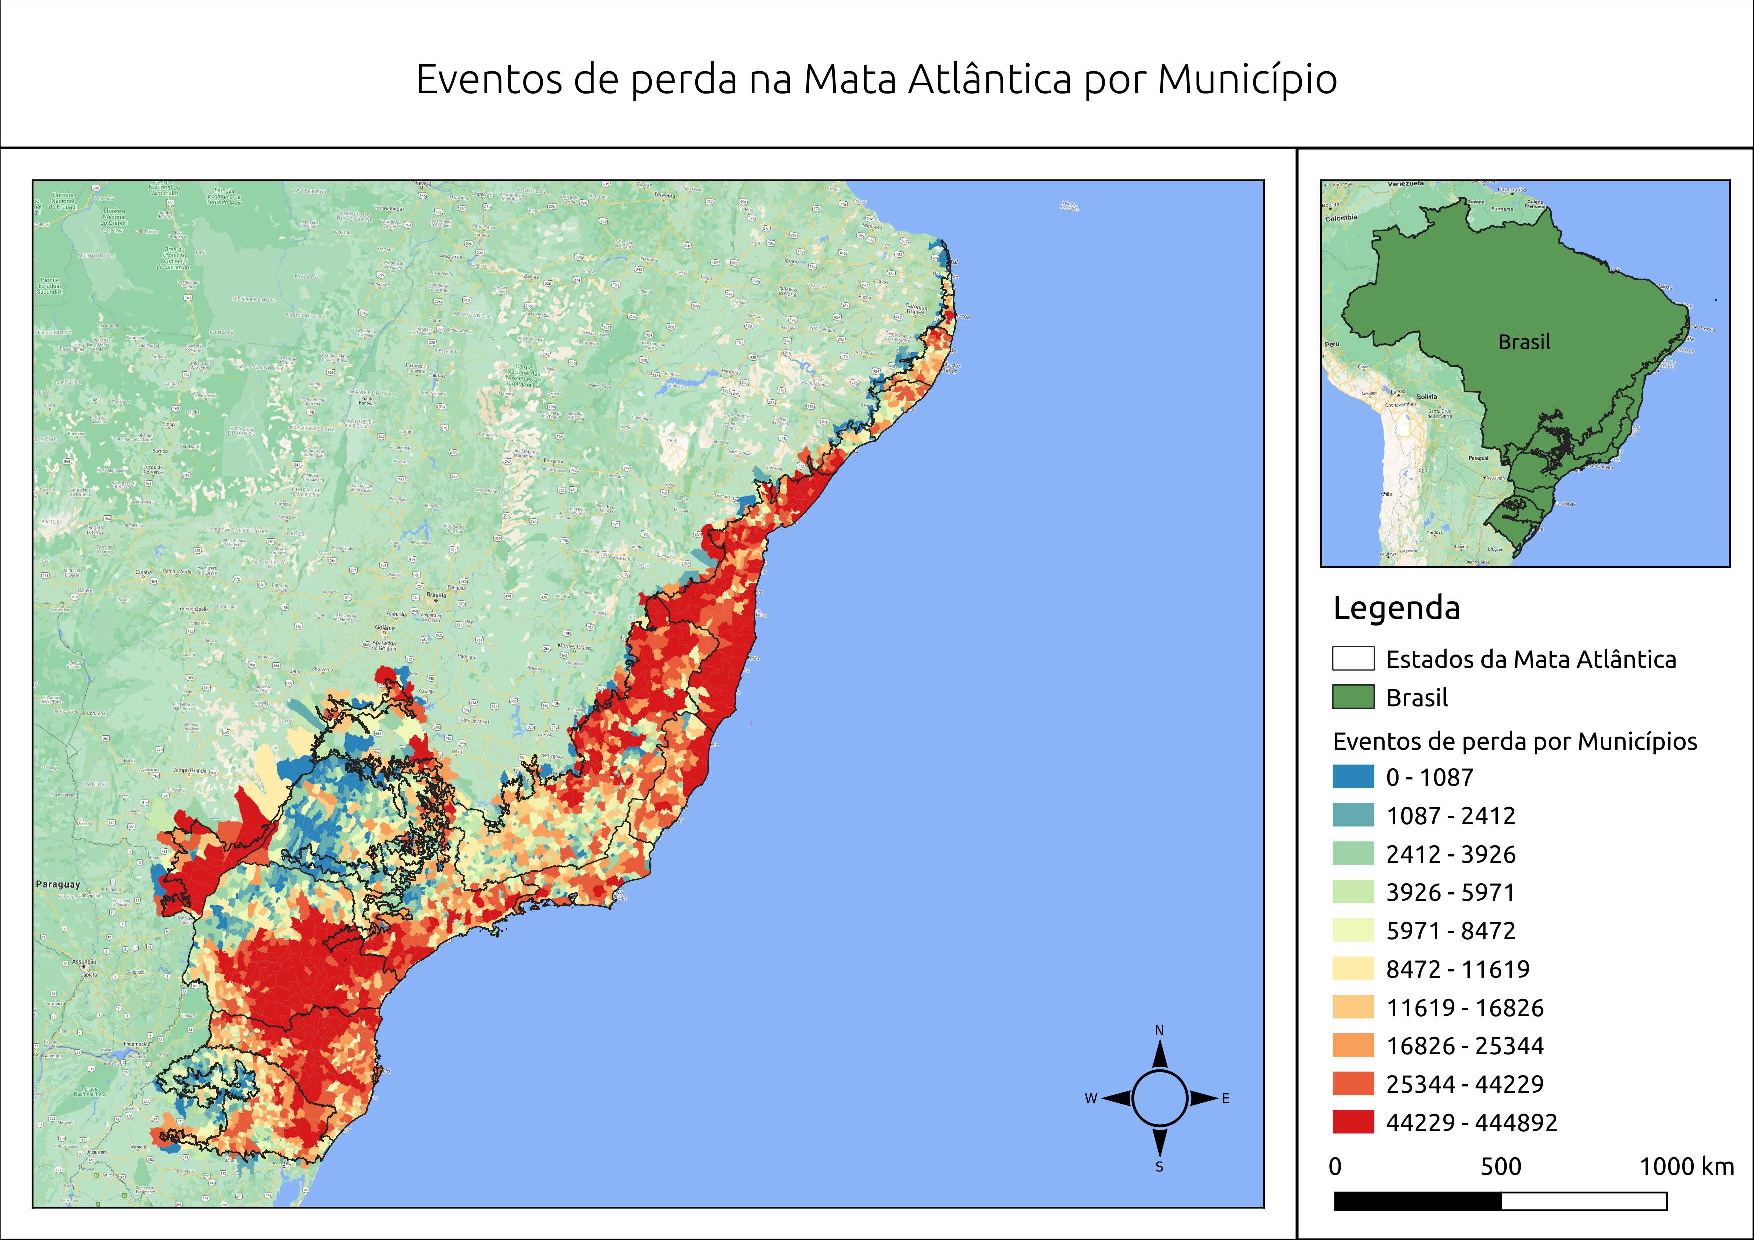
\includegraphics[scale=.5]{images/mun_loss_mun_masked85_maskedgain.pdf}
    \caption{Todos os eventos de perda na Mata Atlântica entre 1985 e 2018 por município. Os valores representam o número de pixels que tiveram alguma detecção de perda.}
    \label{fig:mun_loss_masked85_maskedgain}
\end{figure}

Seja através dos mapas de calor, ou divisões por municípios ou estados, podemos observar que os eventos de perda na Mata Atlântica brasileira ocorre de forma aglomerada em certas regiões. Apesar de termos registrado eventos de perda em todos os tipos de fitofisionomias, parece ter havido uma predominância de eventos em florestas ombrófilas densas principalmente por conta das perdas detectadas no Paraná, Santa Catarina e Bahia.

Podemos observar ainda que grande parte dos eventos de perda no bioma aconteceu durante a década de 1990 concentrados principalmente no sudeste e centro-oeste. Já na parte região sul, os eventos foram mais recentes, ocorrendo em sua maioria durante a década de 2000. Já a região nordeste foi a que mostrou maior variabilidade neste sentido, possuindo estados com eventos mais antigos e recentes (Figura \ref{fig:zonal_loss_yod_byclass}). Ao diminuirmos a escala geográfica da análise para municípios, podemos ver que há, de modo geral, grande presença de eventos durante a década de 1990 em todo o bioma. Mesmo na região sul, boa parte das perdas ocorridas no estado do paraná forma registradas durante esta década (Figura \ref{fig:zonal_mun_loss_yod_byclass}). Nesta escala de análise, podemos observar ainda a presença, mesmo que não proporcionalmente em grande quantidade, de municípios com predominância de perdas bem mais recentes, durante a última década de 2010, principalmente nos estados de Minas Gerais, Paraná, Santa Catarina e São Paulo.

\begin{figure}[H]
    \centering
    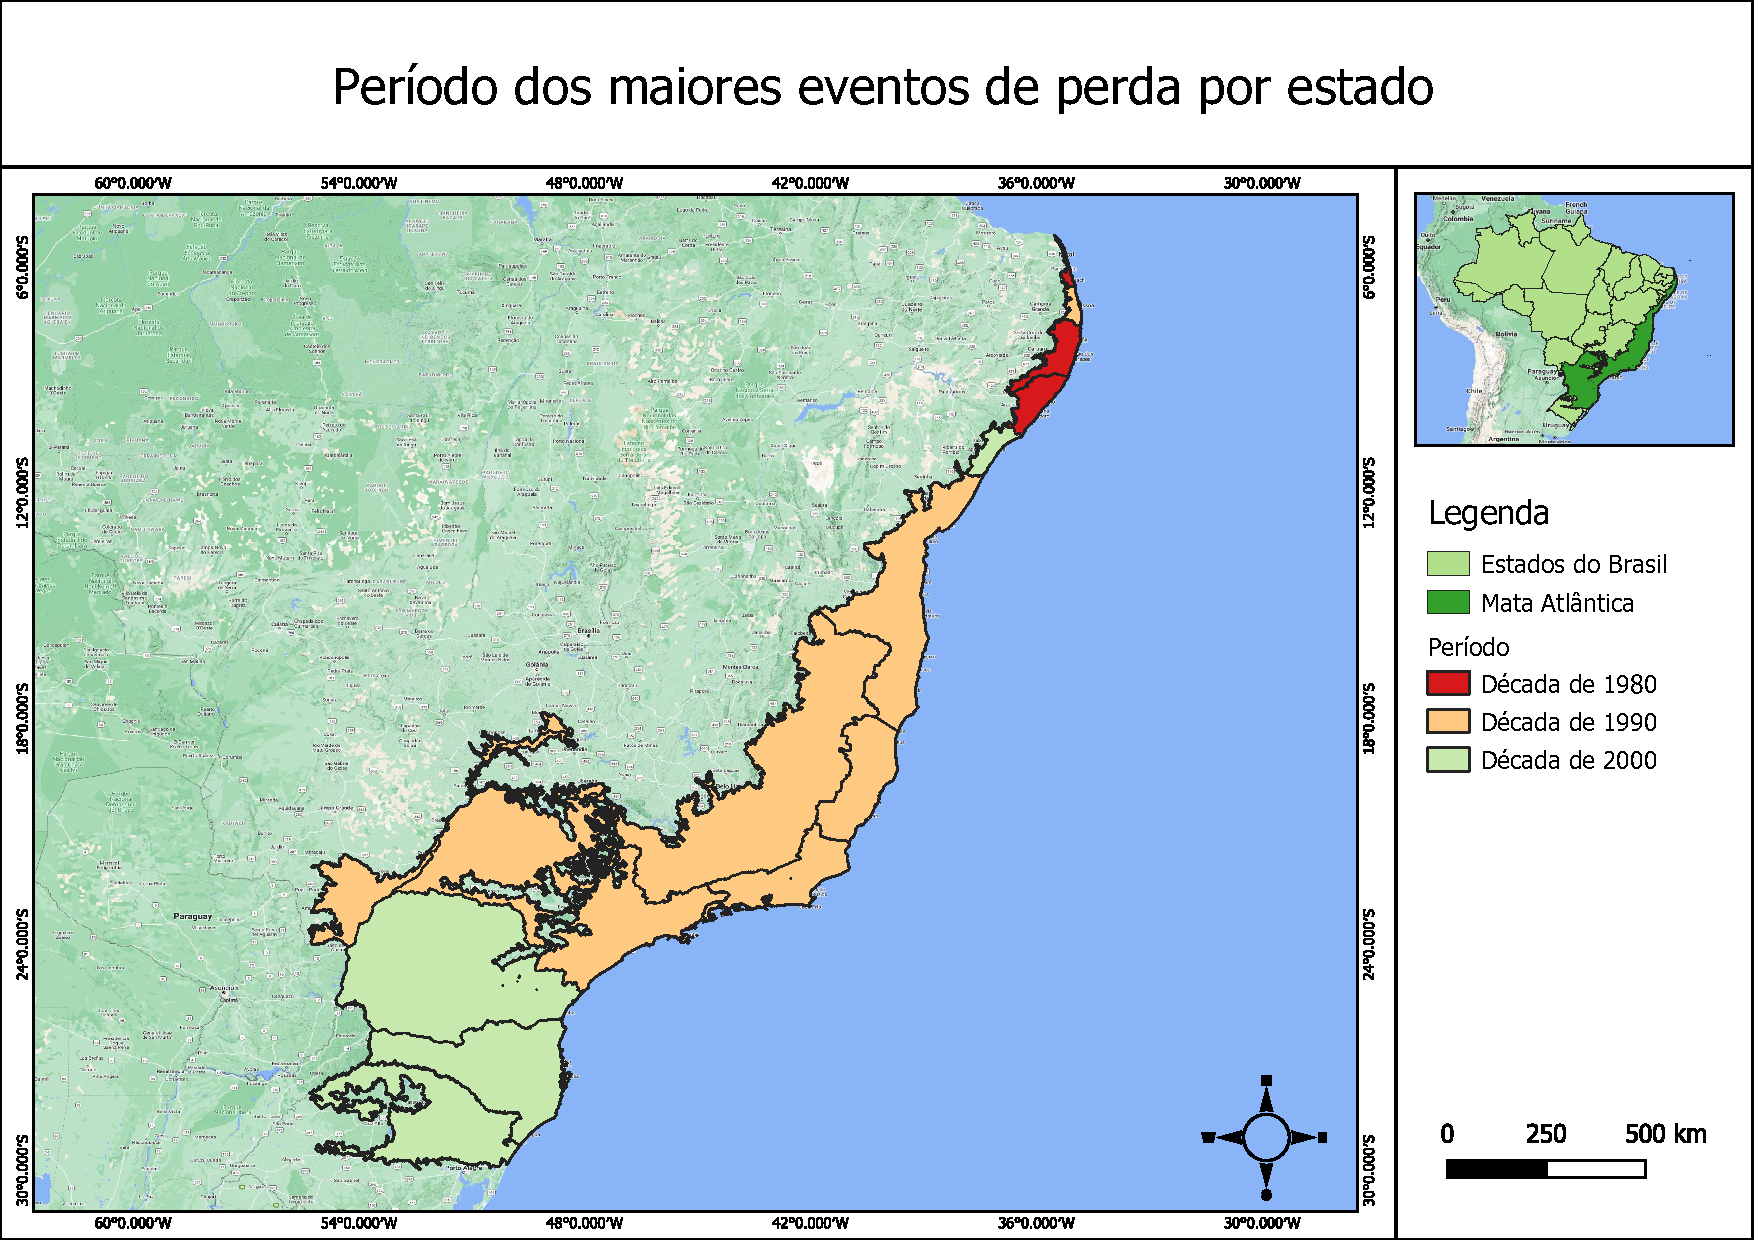
\includegraphics[scale=.5]{images/zonal_loss_yod_byclass.pdf}
    \caption{Mapa com os eventos de perda entre 1985 e 2018 classificado de acordo com a proporção de área de cada estado.}
    \label{fig:zonal_loss_yod_byclass}
\end{figure}

\begin{figure}[H]
    \centering
    \includegraphics[scale=.5]{images/zonal_mun_loss_yod_byclass.pdf}
    \caption{Mapa com os eventos de perda entre 1985 e 2018 classificado de acordo com a proporção de área de cada estado.}
    \label{fig:zonal_mun_loss_yod_byclass}
\end{figure}

O grau de elevação de onde os eventos foram detectados também foram avaliados com o intuito de entender se as mudanças ocorreram em áreas mais altas ou baixas. O modelo digital de elevação utilizado foi o Shuttle Radar Topography Mission (SRTM) com 30m de resolução espacial \citep{srtm30m}. E para a criação da análise foi necessário primeiramente calcular a média da elevação de cada estado, assim como a média dos eventos de mudança e posteriormente subtrair ambos os resultados para a criação de um mapa de elevação relativa:

\begin{equation}
E_{rel} = \frac{1}{n}\sum_{i = 1}^{n} ce_{i} - \frac{1}{n}\sum_{i = 1}^{n} dem_{i} 
\end{equation}

Sendo ($Erel$) a elevação relativa por estado, ($n$) o número de pixel, ($ce$) a camada com os eventos de mudança e ($dem$) a camada original de elevação. Assim, números positivos significam áreas onde a média dos eventos de perda foram detectados acima da elevação média para o estado. Podemos observar na Figura \ref{fig:elev_rel_loss} que todos os estados do sudeste tiveram eventos de perda em áreas mais altas, assim como no estado do Paraná, o que o distoou do resto dos estados do sul que obtiveram média abaixo da elevação, assim como no nordeste.

\begin{figure}[H]
    \centering
    \includegraphics[scale=.5]{images/elev_rel_loss.pdf}
    \caption{Mapa com a elevação relativa dos eventos de perda por estado.}
    \label{fig:elev_rel_loss}
\end{figure}

Além da elevação, foi analisado também o grau de declividade dos eventos de perda com o objetivo de entender se a eventos ocorriam majoritariamente em áreas planas ou com algum grau de declividade. Desta vez a escala de análise se deu no nível de município devido a variabilidade dos dados. Novamente, o dado de entrada para a geração da camada de declividade SRTM 30m \citep{srtm30m}. Os pixels foram agrupados em classes utilizando uma modificação do sistema de classificação de declividade da EMBRAPA 1979 \citep{Embrapaslope} (Figura \ref{fig:slope_loss_byMun}). 

\begin{center}
    \begin{tabular}{ | l | l | }
    \hline
    Declividade (\%) & Relevo \\ \hline
    0 - 3 & Pouco ou nenhum \\ \hline
    4 - 9 & Suave \\ \hline
    10 - 15 & Moderado \\ \hline
    16 - 30 & Íngreme \\ \hline
    31+ & Extremamente Íngreme \\ 
    \hline
    \end{tabular}
\end{center}

É possível observar uma predominância de eventos de declividade íngreme em todo o bioma, com exceção de parte da costa onde a declividade não passou dos 3\% e de regiões no sul/sudeste e norte da Bahia com a presença de inclinações suaves. De forma geral, foi possível observar que a maior parte dos eventos de perda aconteceram em relevos mais inclinados, o que pode demonstrar uma possível procura por novas áreas fora das planícies já desmatadas. 

\begin{figure}[H]
    \centering
    \includegraphics[scale=.5]{images/slope_loss_byMun.pdf}
    \caption{Mapa com os graus de declividade mais comuns de acordo com as áreas de evento de perda para cada município do bioma.}
    \label{fig:slope_loss_byMun}
\end{figure}

\subsubsection{Os eventos de ganho na Mata Atlântica}

\hspace{13pt} Somando-se todos os eventos de ganho detectados pelo algoritmo e após as filtragens necessárias, houveram ao longo de todos os anos da análise 68.869.908 de pixels com um ganho médio de 197 ou aumento de 0.197 no índice NDVI. Isso equivale a uma área total de aproximadamente 62 mil $ km^2 $ de florestas que sofreram ganhos significativos. Como discutido na sessão 3.2.4, áreas de florestas pseudo-invariantes não foram consideradas, sendo assim, esta área representa um ganho real de área verde dentro do bioma. 

Na Figura \ref{fig:heat_gain}, podemos ver que o ganho de áreas no bioma de deu de forma bem mais homogênea que as áreas de perda. Apenas alguns pontos de aglomeração podem ser visualizados como no sul do Rio Grande do Sul, Espírito Santo, sul de Pernambuco, São Paulo e Minas Gerais.

\begin{figure}[H]
    \centering
    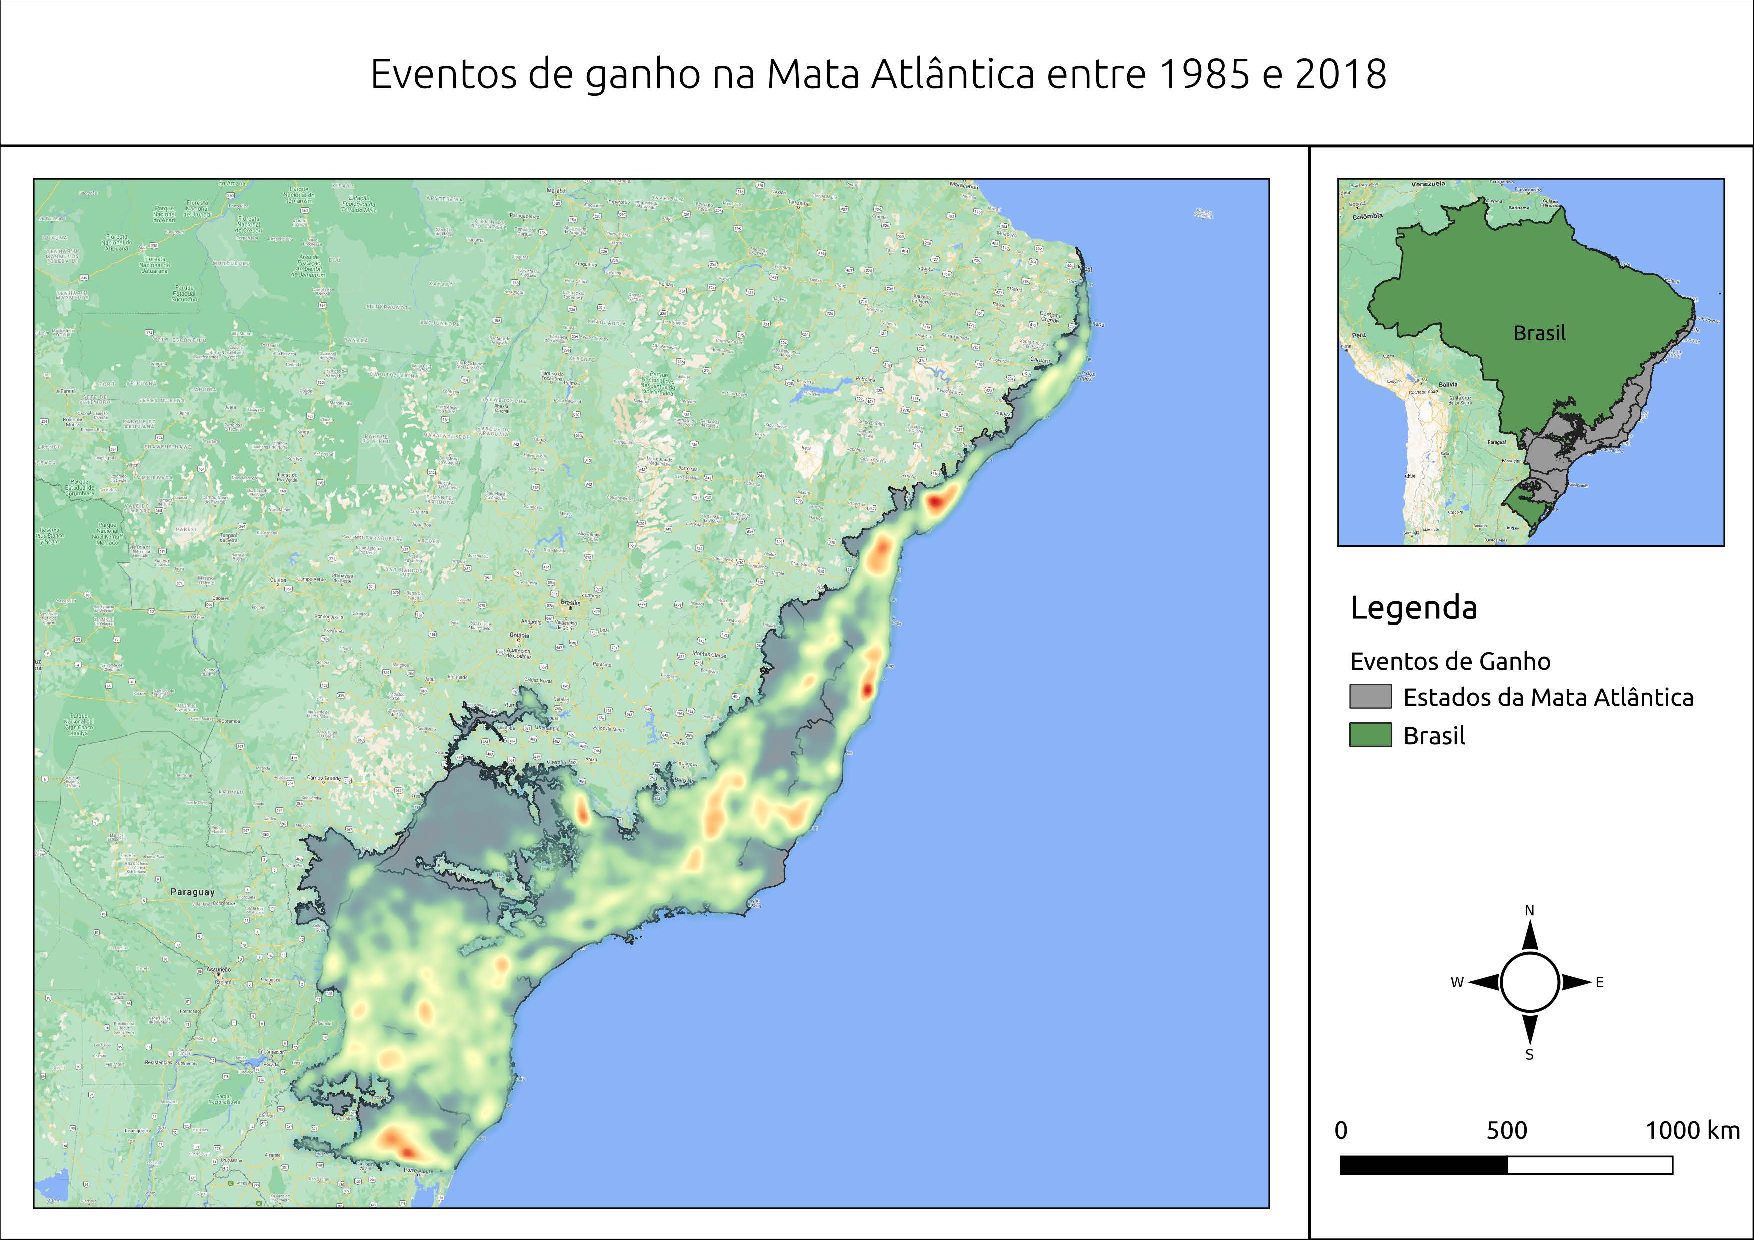
\includegraphics[scale=.5]{images/heatmap_gain_masked18_dur_gt4_inv_for.pdf}
    \caption{Mapa com os eventos de ganho entre 1985 e 2018.}
    \label{fig:heat_gain}
\end{figure}

Quando analisamos por estado, verificamos que Paraná e Minas Gerais dominam na quantidade total de eventos, seguido de São Paulo, Santa Catarina e Bahia (Figura \ref{fig:estados_gain}). Ao dividir o número de eventos pela área de cada estado vemos que o concentração ocorre principalmente em Santa Catarina e Bahia, seguida de Sergipe, Rio Grande do Sul e Espírito Santo (Figura \ref{fig:estados_gain_proporcional}). Assim como nos eventos de perda, ao calcular a proporção dos eventos de ganho por município de acordo com a quantidade original de floresta presente em 1985, o litoral sul e sudeste apresentam baixa proporção de ganho com aumento significativo em regiões do Paraná, São Paulo, Minas Gerais e Bahia (Figura \ref{fig:prop_gain}). O município de Cosmorama em São Paulo foi o recordista no aumento proporcional de área de floresta, saindo de 1,2 km2 em 1985 para 10,4 km2 em 2018, um aumento de aproximadamente 8,6 vezes.

\begin{figure}[H]
    \centering
    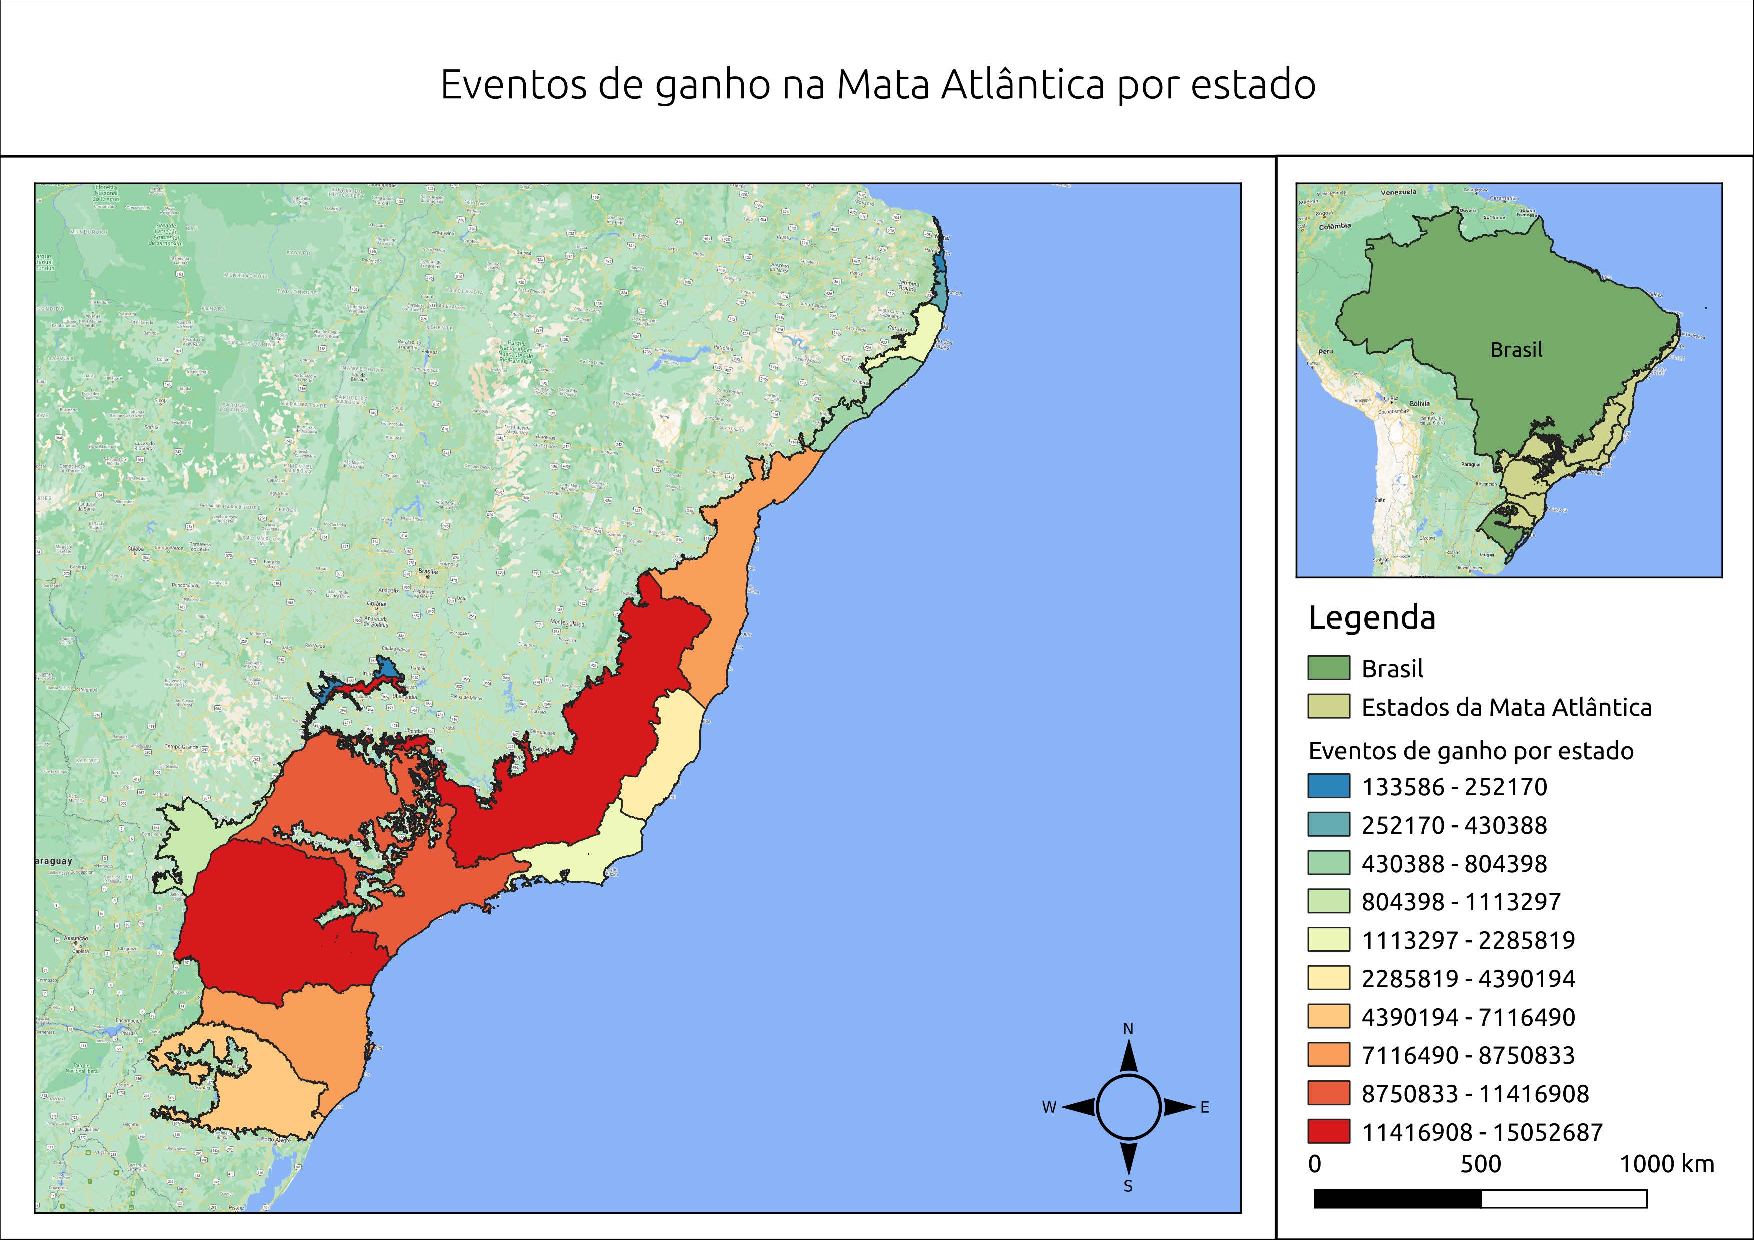
\includegraphics[scale=.5]{images/estados_gain_seg6_masked18_dur_gt4_inv_for.pdf}
    \caption{Mapa com os eventos de ganho entre 1985 e 2018 por estado. Os valores representam o número de pixels que tiveram alguma detecção de ganho.}
    \label{fig:estados_gain}
\end{figure}

\begin{figure}[H]
    \centering
    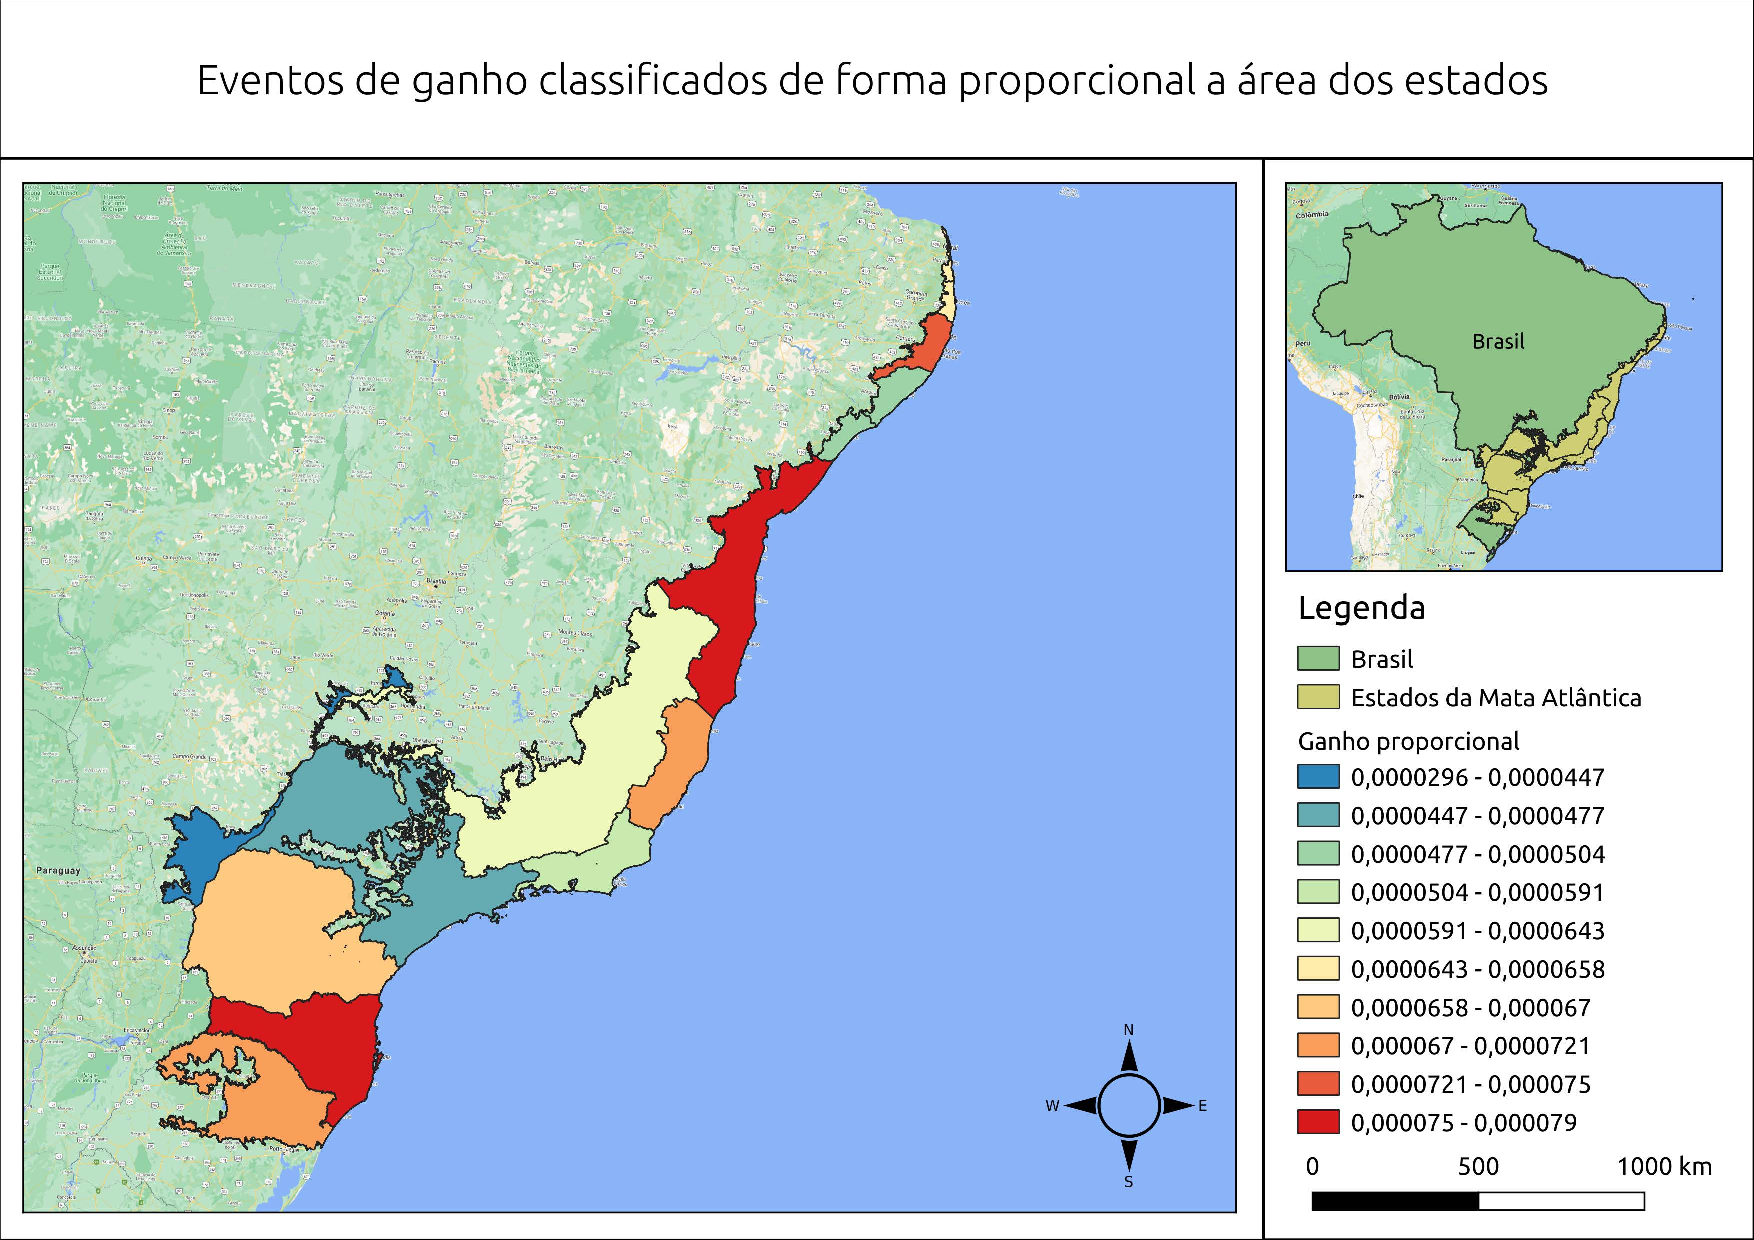
\includegraphics[scale=.5]{images/estado_gain_proporcional.pdf}
    \caption{Mapa com os eventos de ganho entre 1985 e 2018 classificado de acordo com a proporção de área de cada estado.}
    \label{fig:estados_gain_proporcional}
\end{figure}

\begin{figure}[H]
    \centering
    \includegraphics[scale=.5]{images/prop_gain.pdf}
    \caption{Mapa com a proporção dos eventos de ganho entre 1985 e 2018 classificado de acordo com a área total de floresta em 1985.}
    \label{fig:prop_gain}
\end{figure}

Ao analisar a proporção de área ganha dentro das unidades de conservação (UC) presente no bioma, percebemos que, como esperado, a proporção de área ganha dentro das unidades é muito mais significativa que as de perda. Diferente dos cenário de perda, aqui encontramos a média dos anos de início do ganho próximos do início da década de 1990, enquanto na perda a média tende mais para a segunda metade da década ou até mesmo os anos 2000 (Tabela \ref{tab:uc_gain}). 

\begin{table}[H]
    \centering
    \rowcolors{2}{red!50!yellow!30}{green!40!yellow!10}
    % \footnotesize
    \begin{tabular}{|c | c | c | c | c|}
    \hline
            Unidade de Conservação & UF & \% de ganho de área  & Ano Criação & Média YOD \\
                PARNA do Descobrimento & BA & 0.64 & 1999 & 1991 \\ 
                REBIO do Córrego Grande & ES & 0.53 & 1989 & 1989 \\
                ESEC de Aracuri-Esmeralda & RS & 0.44 & 1981 & 1993 \\
                FLONA de Nísia Floresta & RN & 0.43 & 2001 & 1990 \\
                FLONA do Rio Preto & ES & 0.34 & 1990 & 1989 \\
                FLONA de Lorena & SP & 0.23 & 2001 & 1991 \\
                PARNA de Monte Pascoal & BA & 0.22 & 1961 & 1991 \\
                FLONA de Ipanema de Paula & SP & 0.21 & 1992 & 1989 \\
                PARNA do Pau Brasil & BA & 0.18 & 1999 & 1991 \\
                REBIO de Sooretama & ES & 0.17 & 1982 & 1989 \\
    \hline
    \end{tabular}
    \caption{As dez unidades de conservação com maior proporção de ganho de área.}
    \label{tab:uc_gain}
\end{table}

Já quando realizamos a análise de ganho por município, assim como no cenário de perdas, conseguimos perceber uma maior aglomeração em municípios em estados que tiveram baixa taxa de eventos como o Rio de Janeiro (Figura \ref{fig:mun_gain}). A lista de municípios com a maior quantidade de eventos se mostrou um pouco mais heterogênea que a do cenário de perdas (Tabela \ref{tab:mun_gain}). 

\begin{figure}[H]
    \centering
    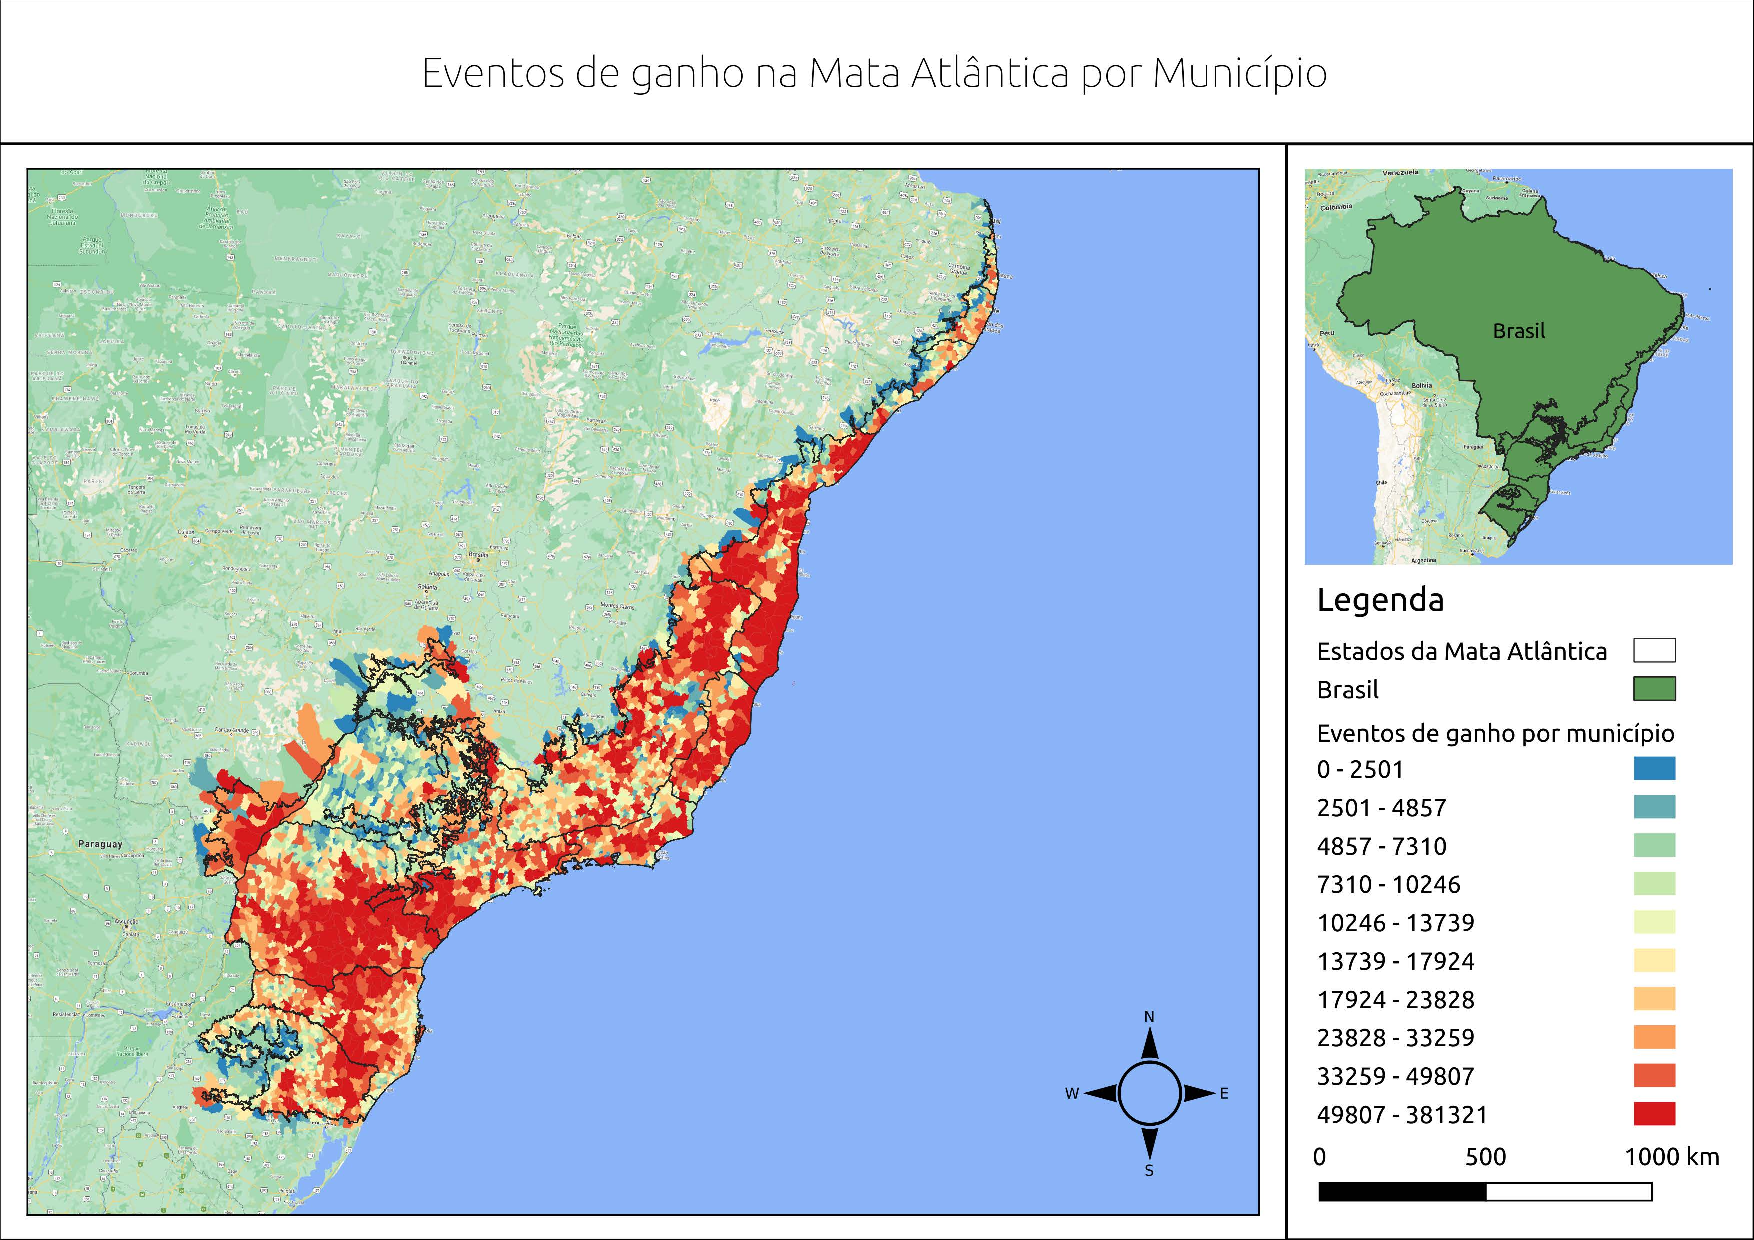
\includegraphics[scale=.5]{images/mun_gain_seg6_masked18_dur_gt4_inv_for.pdf}
    \caption{Mapa com os eventos de ganho entre 1985 e 2018 por município. Os valores representam o número de pixels que tiveram alguma detecção de ganho.}
    \label{fig:mun_gain}
\end{figure}

\begin{table}[H]
    \centering
    \rowcolors{2}{red!50!yellow!30}{green!40!yellow!10}
    % \footnotesize
    \begin{tabular}{|c | c | c|}
    \hline
                            Nome & Eventos & UF \\
                Porto Seguro & 381321 & BA \\ 
                       Prado & 337864 & BA \\
                Jequitinhonha & 309792 & MG \\
        Santa Cruz Cabrália & 243153 & BA \\
                    Linhares & 241735 & ES \\
                      Almenara & 235791 & MG \\
              Prudentópolis & 231492 & PR \\
                    Belmonte & 228173 & BA \\
                  Guarapuava & 225197 & PR \\
                  Ortigueira & 218987 & PR \\
                  Entre Rios & 203945 & BA \\
                   Cruz Machado & 196431 & PR \\
            Domingos Martins & 182013 & ES \\
                 Juiz de Fora & 181554 & MG \\
                   Esplanada & 181265 & BA \\
                      Mariana & 177423 & MG \\
               Teófilo Otoni & 176573 & MG \\
                      Tibagi & 175646 & PR \\
  São Sebastião do Paraíso & 175471 & MG \\
                   Caravelas & 174156 & BA \\
    \hline
    \end{tabular}
    \caption{Os vinte municípios com maior número de eventos de perda}
    \label{tab:mun_gain}
\end{table}

Ao analisar o ano de detecção dos ganhos agregando através das décadas, percebemos que grande parte dos estados tiveram seus ganhos iniciados na década de 1990 com exceção de Sergipe, que apresentou recuperações na década de 1980 (Figura \ref{fig:zonal_gain_yod_byclass}). Ao subdividirmos a análise por municípios, percebemos a presença de recuperações mais recentes espalhadas principalmente em São Paulo, Paraná, Mato Grosso e Minas Gerais. Eventos mais antigos iniciados na década de 1980 também são maioria em alguns municípios em Santa Catarina, São Paulo e Bahia, mas ainda sim, em menor quantidade (Figura \ref{fig:zonal_mun_gain_yod_byclass}).  

\begin{figure}[H]
    \centering
    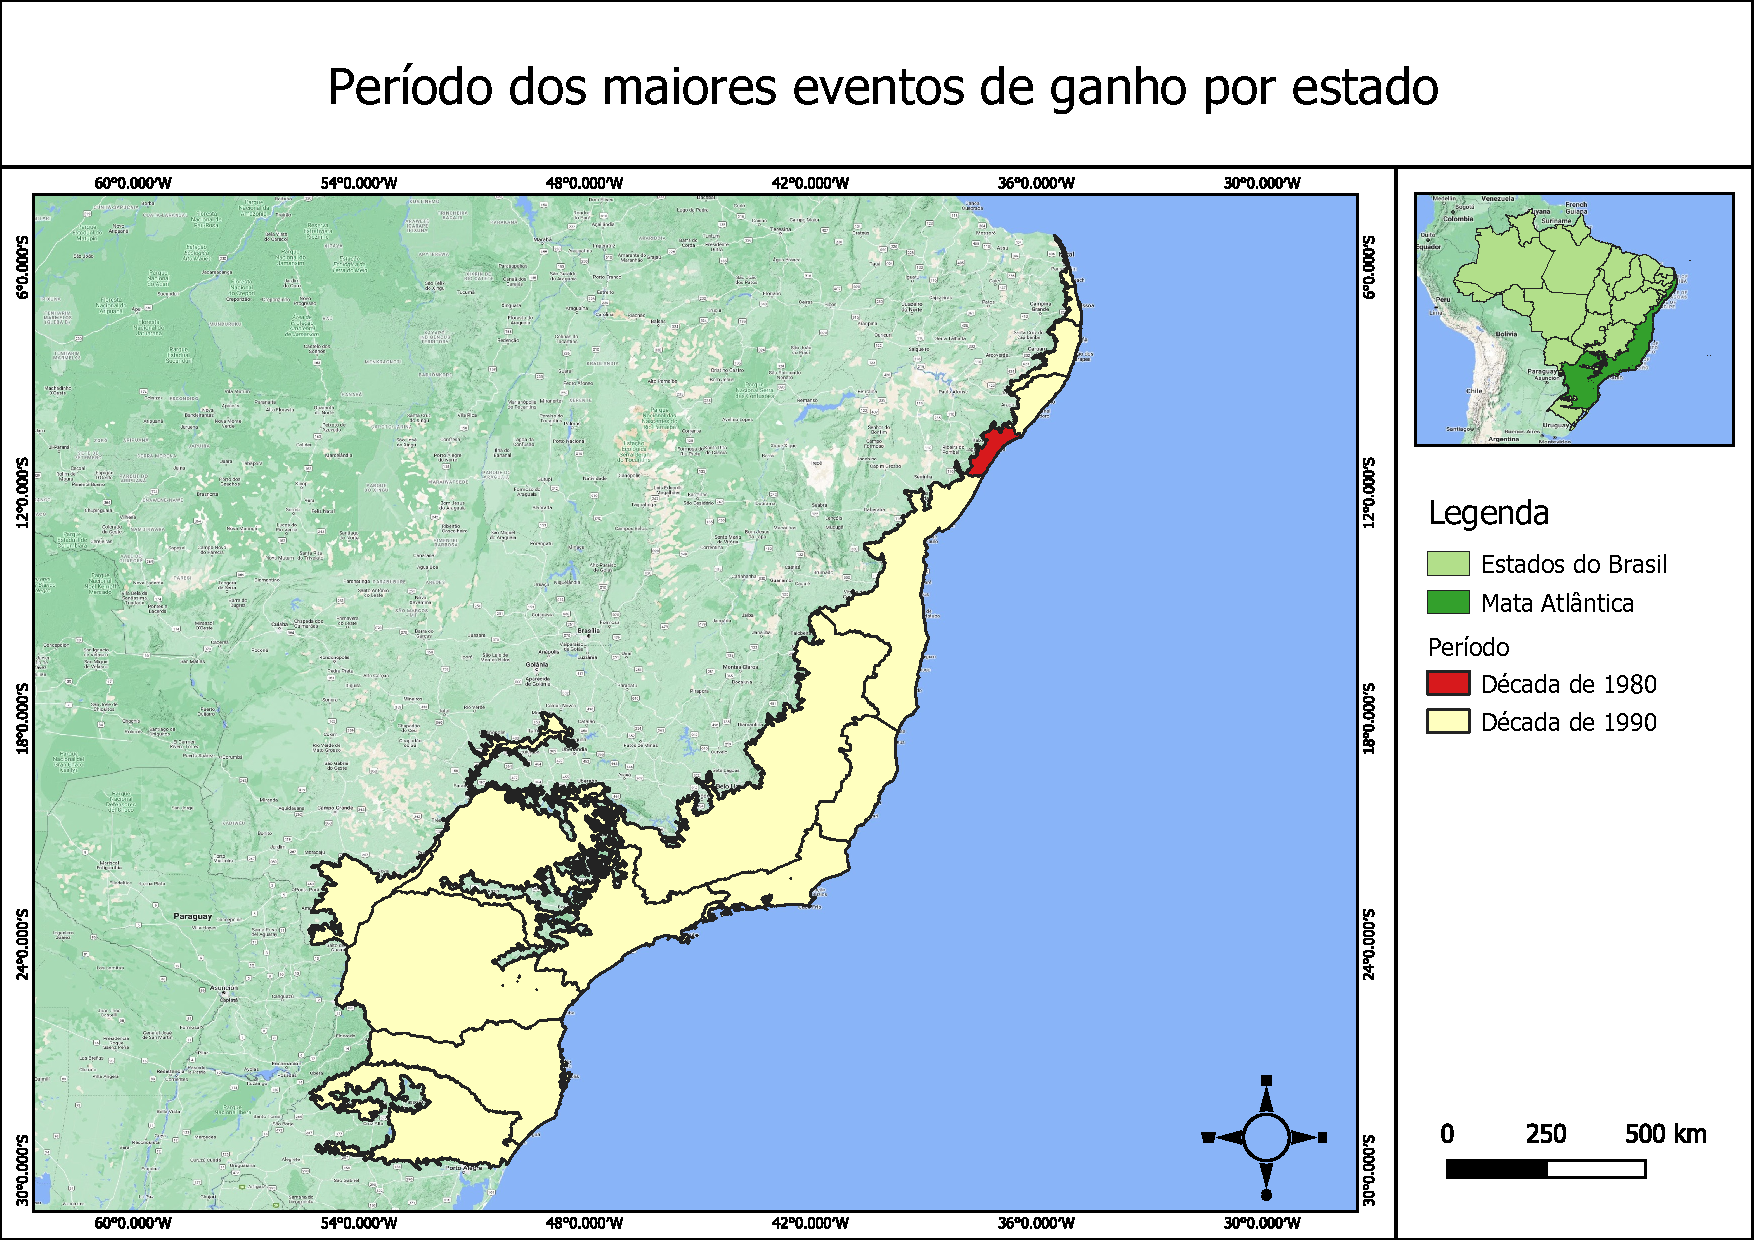
\includegraphics[scale=.5]{images/zonal_gain_yod_byclass.pdf}
    \caption{Mapa com os períodos dos maiores eventos de ganho dividido por década por estado.}
    \label{fig:zonal_gain_yod_byclass}
\end{figure}

\begin{figure}[H]
    \centering
    \includegraphics[scale=.5]{images/zonal_mun_gain_yod_byclass.pdf}
    \caption{Mapa com os períodos dos maiores eventos de ganho dividido por década por município.}
    \label{fig:zonal_mun_gain_yod_byclass}
\end{figure}

Assim como para os eventos de perda, uma análise de elevação foi realizada para identificar estados que tiveram mudanças maiores ou menores que a média da elevação estadual. São Paulo, Rio de Janeiro e Espírito Santo tiveram as maiores médias, mostrando que os eventos de ganho nessas regiões ocorreram em partes mais altas (Figura \ref{fig:elev_rel_gain}). É interessante observar que a região sudeste como um todo obteve uma média alta tanto nos eventos de ganho quanto nos de perda, o que demonstra uma dinâmica maior das partes mais altas. Já no Sul houve uma queda geral da média em relação ao cenário de perda. Já as regiões nordeste e centro-oeste se mantiveram estáveis em todos os estados. 

Já o grau de declividade para os cenários de ganho permaneceu similar ao cenário de perdas, mostrando uma coerência geral. No entanto, é perceptível em certas regiões uma maior quantidade de municípios com grau de declividade maior nos eventos de ganho (Figura \ref{fig:slope_gain_byMun}).

\begin{figure}[H]
    \centering
    \includegraphics[scale=.5]{images/elev_rel_gain.pdf}
    \caption{Mapa com a elevação relativa dos eventos de ganho por estado.}
    \label{fig:elev_rel_gain}
\end{figure}

\begin{figure}[H]
    \centering
    \includegraphics[scale=.5]{images/slope_gain_byMun.pdf}
    \caption{Mapa com os graus de declividade mais comuns de acordo com as áreas de evento de ganho para cada município do bioma.}
    \label{fig:slope_gain_byMun}
\end{figure}

\subsection{Conclusão}

\hspace{13pt} O estudo da paisagem através da análise de séries temporais de imagens orbitais se mostrou essencial para o melhor entendimento dos processos ocorridos em uma região tão importante como a Mata Atlântica. Mesmo sendo um dos biomas mais estudados do pais, a compreensão dos processos de mudança do uso e cobertura do solo através de uma representação visual e a possibilidade da quantificação dos processos só passaram a ser viáveis recentemente. O trabalho apresentou resultados que podem contribuir com projetos de análise e monitoramento do bioma, assim como estudos futuros sobre as mudanças ocorridas nos últimos mais de 30 anos. 

O algoritmo Landtrendr e sua implementação na plataforma Google Earth Engine se mostrou robusto o suficiente para analisar áreas extensas como a do bioma e seus 15 estados com altíssimo rendimento de velocidade de processamento. Ademais, o algoritmo apresentou alto rendimento ao apresentar resultados com acurácia global de 87\% e índice kappa de 0.8. O uso da ferramenta através de \textit{templates} possui ainda capacidade de ampliar sua utilização para públicos ainda maiores e certamente de sua aplicação em ambientes tropicais com qualidade similar aos estudos em áreas temperadas, onde originalmente foi desenvolvido, testado e aplicado.

Apesar da facilidade de uso do Landtrendr em plataformas como o GEE, não se pode dizer que a aplicação do algoritmo é trivial, já que o mesmo possui um custo de processamento elevado mesmo na plataforma do Google. Esta característica acaba gerando a necessidade de códigos um pouco mais complexos, uma capacidade de armazenamento maior e um tempo total de processamento relativamente alto. No entanto, quando comparado a técnicas mais tradicionais, a utilização da técnica ainda apresenta benefícios significativos. Todo o trabalho de pré-processamento e criação de composições processadas como dado de entrada é feito com apenas uma única função, e a escolha dos parâmetros pode ser feita de forma rápida tanto dentro da plataforma como em aplicativos web criados especialmente para a realização de testes. 

Quanto aos resultados obtidos, os resultados mostraram um bioma com mais ganhos do que perdas de áreas florestadas. Grande parte dos eventos de ganho podem ser considerados antigos, iniciados ainda na década de 1990, mas como foi possível observar, existe boa parte do território com áreas de floresta secundária mais recentes, com menos de 20 anos de existência. No geral, foram detectados na última década mais eventos de ganho (11,667 km2) do que de perda (8,796 km2). Estados como o do Paraná e de Santa Catarina tiveram ao mesmo tempo uma boa quantidade de eventos de ganho quanto também de perda com idade similar, o que demonstra alta dinâmica na mudança do uso e cobertura na região.

Grande parte dos eventos foram detectados em áreas com declividade considerada íngreme em todo o bioma. Isso pode ser um indicativo de disputas por terras em regiões menos estabelecidas. Já grande parte da região sul, centro-oeste e nordeste, declividades mais baixas foram majoritárias, o que pode significar mudanças em remanescentes já altamente fragmentados existentes nas planícies com presença de áreas cultivadas. Outro resultado significativo foi a dominância de eventos de mudança em áreas mais elevadas que a média principalmente no sudeste, o que pode ser indicativo de uma maior mudança em áreas chave para importantes para a manutenção de bacias hidrográficas e outros serviços ecossistêmicos.

Este trabalho teve como objetivo utilizar o algoritmo Landtrendr para contribuir para um maior entendimento sobre o bioma da Mata Atlântica e consequentemente para programas e projetos de conservação e restauração de uma região que é um \textit{hotspot} de biodiversidade. O espaço temporal escolhido também possui sua importância devido a sua relevância social e política, vide que representa um momento chave de reestabelecimento da democracia brasileira. O bioma foi o primeiro a ser colonizado e povoado, possui até hoje a maior quantidade da população nacional e um das paisagens mais fragmentadas dentre todos os biomas. No entanto, como os resultados indicam, é um bioma que pode representar a esperança necessária para a conservação e restauração que o pais precisa como busca para um desenvolvimento, de fato, sustentável. 

